% ============================================================
%  Network Security -- Module 1: Foundations of Network Security
%  Lesson 1: Introduction to Network Security
%  Lesson 2: Network Models
%  Beamer (Madrid theme). Compile with: pdflatex module1.tex (twice)
% ============================================================
\documentclass[aspectratio=169,11pt,xcolor={table}]{beamer}
\usetheme{Madrid}
\usefonttheme{professionalfonts}

\usepackage[T1]{fontenc}
\usepackage{lmodern}
\usepackage{booktabs}
\usepackage{array}
\usepackage{tikz}
\usetikzlibrary{arrows.meta,positioning,shapes.geometric,shapes.symbols,
  shapes.misc,shadows,calc,fit,backgrounds,mindmap,decorations.pathmorphing,decorations.pathreplacing}

% ------------------------------------------------------------
%  Colour palette
% ------------------------------------------------------------
\definecolor{navy}{RGB}{21,45,99}
\definecolor{ocean}{RGB}{28,97,158}
\definecolor{aqua}{RGB}{0,142,150}
\definecolor{brick}{RGB}{200,55,45}
\definecolor{amber}{RGB}{235,150,20}
\definecolor{leaf}{RGB}{40,160,90}
\definecolor{grape}{RGB}{125,70,165}
\definecolor{sky}{RGB}{235,243,252}
\definecolor{ink}{RGB}{40,40,50}

\setbeamercolor{palette primary}{bg=ocean,fg=white}
\setbeamercolor{palette secondary}{bg=navy!85,fg=white}
\setbeamercolor{palette tertiary}{bg=navy,fg=white}
\setbeamercolor{palette quaternary}{bg=navy,fg=white}
\setbeamercolor{structure}{fg=ocean}
\setbeamercolor{title}{bg=navy,fg=white}
\setbeamercolor{frametitle}{bg=navy,fg=white}
\setbeamercolor{block title}{bg=ocean,fg=white}
\setbeamercolor{block body}{bg=sky,fg=ink}
\setbeamercolor{block title alerted}{bg=brick,fg=white}
\setbeamercolor{block body alerted}{bg=brick!8,fg=ink}
\setbeamercolor{block title example}{bg=leaf,fg=white}
\setbeamercolor{block body example}{bg=leaf!8,fg=ink}
\setbeamercolor{normal text}{fg=ink}
\setbeamercolor{alerted text}{fg=brick}
\setbeamercolor{item projected}{bg=ocean,fg=white}
\setbeamertemplate{items}[circle]
\setbeamertemplate{blocks}[rounded][shadow=true]
\setbeamertemplate{navigation symbols}{}

% Section divider slide
\AtBeginSection[]{
  \begin{frame}[plain]
    \begin{tikzpicture}[remember picture,overlay]
      \fill[navy] (current page.south west) rectangle (current page.north east);
      \fill[ocean] (current page.south west) rectangle ([yshift=1.2cm]current page.south east);
      \fill[aqua] ([yshift=1.2cm]current page.south west) rectangle ([yshift=1.35cm]current page.south east);
      \foreach \i in {1,...,6}
        \draw[white,opacity=0.06,line width=14pt]
          ([xshift=\i*1.6cm]current page.north west) circle (\i*0.9cm);
      \node[white,font=\large,anchor=west] at ([xshift=1.2cm,yshift=0.9cm]current page.west)
        {Lesson \thesection};
      \node[white,font=\huge\bfseries,anchor=west,text width=12cm] at ([xshift=1.2cm,yshift=-0.1cm]current page.west)
        {\insertsectionhead};
      \node[white,opacity=0.8,anchor=east,font=\small] at ([xshift=-0.8cm,yshift=0.6cm]current page.south east)
        {Module 1 \,$\cdot$\, Foundations of Network Security};
    \end{tikzpicture}
  \end{frame}
}

% ------------------------------------------------------------
%  TikZ styles and small pictograms
% ------------------------------------------------------------
\tikzset{
  >={Stealth[length=2.6mm]},
  box/.style={draw=#1!80!black,fill=#1!15,rounded corners=4pt,thick,
    minimum height=8mm,minimum width=22mm,align=center,font=\small,
    drop shadow={opacity=0.25}},
  box/.default=ocean,
  lay/.style={fill=#1,text=white,rounded corners=3pt,minimum width=38mm,minimum height=9mm,font=\scriptsize,align=center},
  solid box/.style={fill=#1,text=white,rounded corners=4pt,
    minimum height=8mm,minimum width=22mm,align=center,font=\small\bfseries,
    drop shadow={opacity=0.3}},
  solid box/.default=ocean,
  flow/.style={->,very thick,draw=#1},
  flow/.default=ink!70,
  station/.style={circle,draw=#1!80!black,fill=#1!20,very thick,minimum size=13mm,
    font=\small\bfseries,align=center},
  station/.default=ocean,
  tag/.style={font=\scriptsize,text=ink!80,align=center},
  layer/.style={draw=white,thick,fill=#1,text=white,minimum width=40mm,
    minimum height=6.5mm,font=\small\bfseries},
  % pictograms
  pics/pc/.style={code={
    \fill[#1!85!black,rounded corners=1.5pt] (-0.42,-0.05) rectangle (0.42,0.52);
    \fill[white!90!#1] (-0.36,0.01) rectangle (0.36,0.46);
    \fill[#1!85!black] (-0.06,-0.05) rectangle (0.06,-0.18);
    \fill[#1!85!black,rounded corners=1pt] (-0.24,-0.18) rectangle (0.24,-0.24);
  }},
  pics/pc/.default=ocean,
  pics/person/.style={code={
    \fill[#1] (0,0.46) circle (0.16);
    \fill[#1,rounded corners=5pt] (-0.27,-0.1) -- (-0.27,0.2) -- (0.27,0.2) -- (0.27,-0.1) -- cycle;
  }},
  pics/person/.default=ocean,
  pics/lock/.style={code={
    \draw[#1!80!black,line width=2.2pt] (-0.15,0.12) -- (-0.15,0.28) arc (180:0:0.15) -- (0.15,0.12);
    \fill[#1,rounded corners=2pt] (-0.26,-0.22) rectangle (0.26,0.14);
    \fill[white] (0,-0.02) circle (0.05);
    \fill[white] (-0.02,-0.02) rectangle (0.02,-0.13);
  }},
  pics/lock/.default=amber,
  pics/doc/.style={code={
    \fill[white,draw=#1,thick] (-0.25,-0.33) -- (-0.25,0.33) -- (0.12,0.33) -- (0.25,0.2) -- (0.25,-0.33) -- cycle;
    \draw[#1,thick] (0.12,0.33) -- (0.12,0.2) -- (0.25,0.2);
    \foreach \y in {0.12,0,-0.12,-0.24} \draw[#1!70,thick] (-0.16,\y) -- (0.16,\y);
  }},
  pics/doc/.default=ocean,
  pics/key/.style={code={
    \draw[#1,line width=2pt] (0,0) circle (0.12);
    \draw[#1,line width=2pt] (0.12,0) -- (0.5,0) (0.38,0) -- (0.38,-0.12) (0.47,0) -- (0.47,-0.1);
  }},
  pics/key/.default=amber,
}
\newcommand{\comma}{,}
\newcommand{\hl}[1]{\textcolor{ocean}{\textbf{#1}}}
\newcommand{\bad}[1]{\textcolor{brick}{\textbf{#1}}}
\newcommand{\good}[1]{\textcolor{leaf}{\textbf{#1}}}

\makeatletter
% University logo, small, top-right corner of every page
\AddToHook{shipout/foreground}{%
  \put(\strip@pt\paperwidth,0){%
    \makebox(0,0)[tr]{\raisebox{-0.8cm}{
\includegraphics[height=0.72cm]{au_logo.png}\hspace{0.15cm}}}}}
\makeatother

% ------------------------------------------------------------
\title[Module 1: Foundations]{Foundations of Network Security}
\subtitle{Module 1 \,\textbar\, Lesson 1: Introduction to Network Security \,\textbullet\, Lesson 2: Network Models}
\author[Network Security]{Network Security}
\institute[SLM]{Self-Learning Material \,--\, Lessons 1 \& 2}
\date{}

\begin{document}

% ============================================================
\begin{frame}[plain]
  
\begin{tikzpicture}[remember picture,overlay]
    \shade[top color=navy,bottom color=ocean] (current page.south west) rectangle (current page.north east);
    \foreach \i/\o in {1/0.10,2/0.08,3/0.06,4/0.05,5/0.04}
      \draw[white,opacity=\o,line width=1.2pt] ([xshift=-2.5cm,yshift=-0.5cm]current page.north east) circle (\i*1.1cm);
    \fill[aqua] ([yshift=2.35cm]current page.south west) rectangle ([yshift=2.45cm]current page.south east);
    % network motif
    \begin{scope}[shift={([xshift=-3.3cm,yshift=0.6cm]current page.east)},scale=0.9]
      \foreach \a/\n in {90/a,162/b,234/c,306/d,18/e}
        \node[circle,fill=white,opacity=0.9,minimum size=4mm,inner sep=0] (\n) at (\a:1.6) {};
      \node[circle,fill=amber,minimum size=9mm] (h) at (0,0) {};
      \pic[white] at (0,-0.02) {lock=white};
      \foreach \n in {a,b,c,d,e} \draw[white,opacity=0.7,thick] (h) -- (\n);
      \draw[white,opacity=0.5,thick] (a) -- (b) -- (c) -- (d) -- (e) -- (a);
    \end{scope}
    \node[white,anchor=west,font=\normalsize] at ([xshift=1.1cm,yshift=2.4cm]current page.west)
      {NETWORK SECURITY \,\textbar\, MODULE 1};
    \node[white,anchor=west,font=\fontsize{28}{32}\selectfont\bfseries,text width=9.5cm] at ([xshift=1.1cm,yshift=1.0cm]current page.west)
      {Foundations of\\[2pt] Network Security};
    \node[white,opacity=0.9,anchor=west,text width=9cm,font=\small] at ([xshift=1.1cm,yshift=-0.9cm]current page.west)
      {Lesson 1 \,--\, Introduction to Network Security\\ Lesson 2 \,--\, Network Models};
    \node[white,opacity=0.85,anchor=west,font=\footnotesize] at ([xshift=1.1cm,yshift=1.2cm]current page.south west)
      {Cryptography \,$\cdot$\, Attacks \,$\cdot$\, Services \,$\cdot$\, Mechanisms \,$\cdot$\, LAN/MAN/WAN \,$\cdot$\, OSI \& TCP/IP};
  \end{tikzpicture}
\end{frame}

% ============================================================
\begin{frame}{Roadmap of This Module}
  \centering
  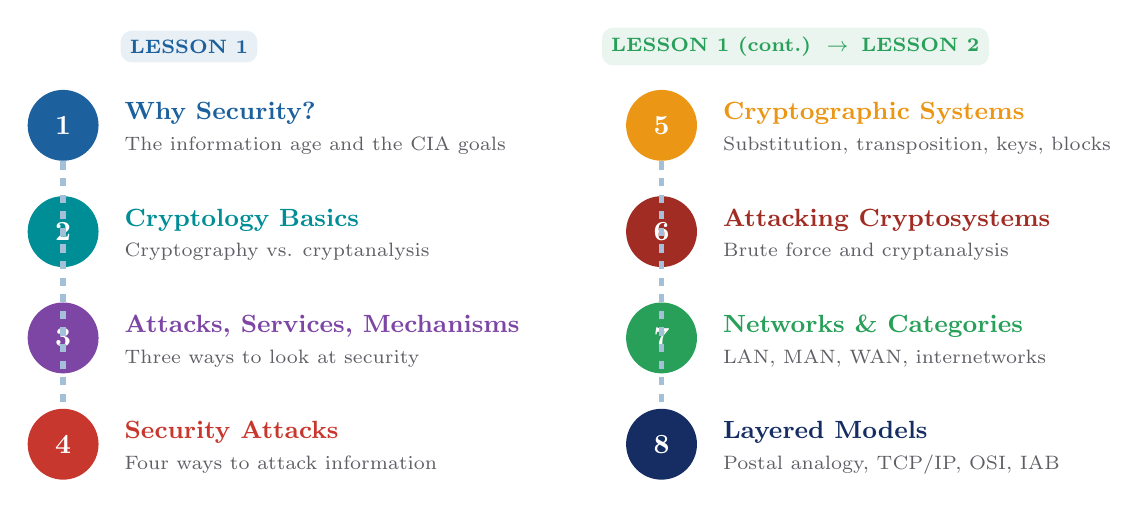
\begin{tikzpicture}[node distance=4mm]
    \foreach \t/\c/\n [count=\i] in {
      Why Security?/ocean/The information age and the CIA goals,
      Cryptology Basics/aqua/Cryptography vs. cryptanalysis,
      Attacks\comma{} Services\comma{} Mechanisms/grape/Three ways to look at security,
      Security Attacks/brick/Four ways to attack information,
      Cryptographic Systems/amber/Substitution\comma{} transposition\comma{} keys\comma{} blocks,
      Attacking Cryptosystems/brick!80!black/Brute force and cryptanalysis,
      Networks \& Categories/leaf/LAN\comma{} MAN\comma{} WAN\comma{} internetworks,
      Layered Models/navy/Postal analogy\comma{} TCP\slash IP\comma{} OSI\comma{} IAB}
    {
      \pgfmathsetmacro{\x}{ifthenelse(\i<5,0,7.6)}
      \pgfmathsetmacro{\y}{-mod(\i-1,4)*1.35}
      \node[circle,fill=\c,text=white,font=\bfseries,minimum size=9mm] (n\i) at (\x,\y) {\i};
      \node[anchor=west,font=\small\bfseries,text=\c] at ([xshift=2mm,yshift=1.5mm]n\i.east) {\t};
      \node[anchor=west,font=\scriptsize,text=ink!75] at ([xshift=2mm,yshift=-2.6mm]n\i.east) {\n};
    }
    \draw[ocean!40,line width=2pt,dashed] (n1) -- (n4);
    \draw[ocean!40,line width=2pt,dashed] (n5) -- (n8);
    \node[fill=ocean!10,rounded corners,font=\scriptsize\bfseries,text=ocean] at (1.6,1.0) {LESSON 1};
    \node[fill=leaf!10,rounded corners,font=\scriptsize\bfseries,text=leaf] at (9.3,1.0) {LESSON 1 (cont.) \,$\rightarrow$\, LESSON 2};
  \end{tikzpicture}
\end{frame}

% ============================================================

% ============================================================
\section{Introduction to Network Security}
% ============================================================

\begin{frame}{We Live in the Information Age}
  \begin{columns}[c]
    \begin{column}{0.52\textwidth}
      \centering
      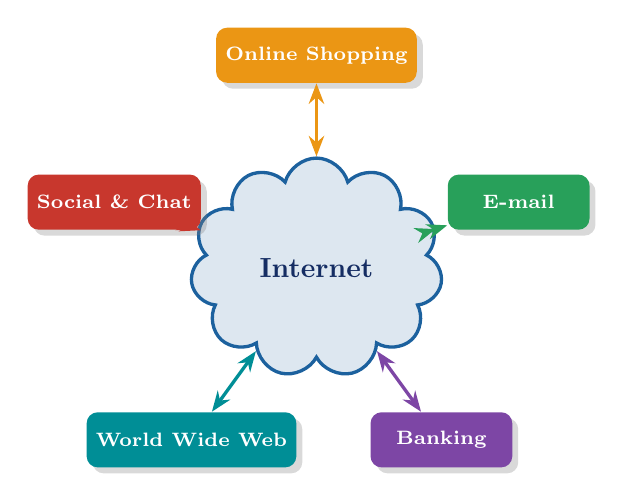
\begin{tikzpicture}
        \node[cloud,cloud puffs=11,draw=ocean,fill=ocean!15,very thick,minimum width=3.2cm,minimum height=2cm,
          font=\bfseries,text=navy] (net) at (0,0) {Internet};
        \foreach \a/\t/\c in {90/Online Shopping/amber,18/E-mail/leaf,-54/Banking/grape,-126/World Wide Web/aqua,162/Social \& Chat/brick}{
          \node[solid box=\c,minimum width=18mm,minimum height=7mm,font=\scriptsize\bfseries] (b\a) at (\a:2.7) {\t};
          \draw[\c,very thick,<->] (net) -- (b\a);
        }
      \end{tikzpicture}
    \end{column}
    \begin{column}{0.46\textwidth}
      \begin{itemize}\setlength{\itemsep}{4pt}
        \item The Internet has changed daily life: \hl{shopping, e-mail, WWW, banking}
        \item This convenience created \bad{dependency} on the Internet
        \item As an \emph{open forum}, the Internet also created security problems
      \end{itemize}
      \vspace{2mm}
      \begin{block}{People need to be sure that\dots}
        \small
        \textbullet~their communication stays \textbf{confidential}\\
        \textbullet~online vendors are \textbf{authentic}\\
        \textbullet~bank requests keep their \textbf{integrity}
      \end{block}
    \end{column}
  \end{columns}
\end{frame}

% ------------------------------------------------------------
\begin{frame}{Information Is an Asset}
  \centering
  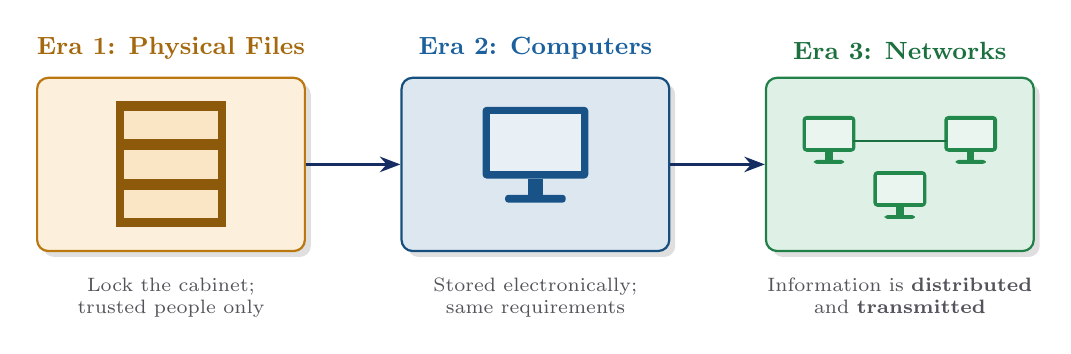
\begin{tikzpicture}[node distance=12mm]
    \node[box=amber,minimum width=34mm,minimum height=22mm] (p) {};
    \node[font=\small\bfseries,text=amber!70!black,above=1mm of p.north] {Era 1: Physical Files};
    \fill[amber!60!black] ([xshift=-7mm,yshift=-8mm]p.center) rectangle ([xshift=7mm,yshift=8mm]p.center);
    \foreach \y in {-5,0,5} \fill[amber!25] ([xshift=-6mm,yshift=\y mm-1.8mm]p.center) rectangle ([xshift=6mm,yshift=\y mm+1.8mm]p.center);
    \node[box=ocean,minimum width=34mm,minimum height=22mm,right=of p] (c) {};
    \node[font=\small\bfseries,text=ocean,above=1mm of c.north] {Era 2: Computers};
    \pic[scale=1.6] at ([yshift=-1mm]c.center) {pc=ocean};
    \node[box=leaf,minimum width=34mm,minimum height=22mm,right=of c] (n) {};
    \node[font=\small\bfseries,text=leaf!70!black,above=1mm of n.north] {Era 3: Networks};
    \pic[scale=0.8] at ([xshift=-9mm,yshift=2mm]n.center) {pc=leaf};
    \pic[scale=0.8] at ([xshift=9mm,yshift=2mm]n.center) {pc=leaf};
    \pic[scale=0.8] at ([yshift=-5mm]n.center) {pc=leaf};
    \draw[leaf!70!black,thick] ([xshift=-6mm,yshift=3mm]n.center) -- ([xshift=6mm,yshift=3mm]n.center);
    \draw[flow=navy] (p) -- (c);
    \draw[flow=navy] (c) -- (n);
    \node[tag,below=2mm of p,text width=34mm] {Lock the cabinet;\\trusted people only};
    \node[tag,below=2mm of c,text width=34mm] {Stored electronically;\\same requirements};
    \node[tag,below=2mm of n,text width=34mm] {Information is \textbf{distributed}\\and \textbf{transmitted}};
  \end{tikzpicture}
  \vspace{3mm}
  \begin{block}{Key idea}
    Information is an \textbf{asset} with value like any other asset. It must be \textbf{hidden} from unauthorized
    access, \textbf{protected} from unauthorized change, and \textbf{available} to authorized users.
    The requirements stayed the same, but in networks they must hold \emph{both at rest and in transit}.
  \end{block}
\end{frame}

% ------------------------------------------------------------
\begin{frame}{Computer, Network and Internet Security}
  \begin{columns}[c]
    \begin{column}{0.48\textwidth}
      \centering
      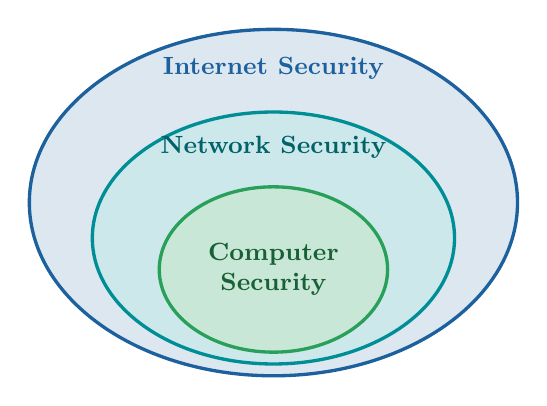
\begin{tikzpicture}
        \fill[ocean!15,draw=ocean,very thick] (0,0) ellipse (3.1cm and 2.2cm);
        \fill[aqua!20,draw=aqua,very thick] (0,-0.45) ellipse (2.3cm and 1.6cm);
        \fill[leaf!25,draw=leaf,very thick] (0,-0.85) ellipse (1.45cm and 1.05cm);
        \node[font=\small\bfseries,text=ocean] at (0,1.7) {Internet Security};
        \node[font=\small\bfseries,text=aqua!70!black] at (0,0.7) {Network Security};
        \node[font=\small\bfseries,text=leaf!60!black,align=center] at (0,-0.85) {Computer\\Security};
      \end{tikzpicture}
    \end{column}
    \begin{column}{0.5\textwidth}
      \begin{description}\setlength{\itemsep}{5pt}
        \item[\textcolor{leaf!70!black}{Computer security}] Tools that protect data stored on a computer and stop hackers
        \item[\textcolor{aqua!70!black}{Network security}] Measures that protect data \textbf{during transmission}
        \item[\textcolor{ocean}{Internet security}] Measures to \textbf{prevent, detect and correct} violations across a collection of interconnected networks
      \end{description}
      \vspace{2mm}
      \begin{alertblock}{No clear boundaries}
        \small A virus may arrive on a disk \emph{or} over the network. Once it is resident, computer-security tools must detect and remove it.
      \end{alertblock}
    \end{column}
  \end{columns}
\end{frame}

% ------------------------------------------------------------
\begin{frame}{Two Examples of Security Violations}
  \begin{columns}[T]
    \begin{column}{0.49\textwidth}
      \centering\textbf{\textcolor{ocean}{Example 1: Disclosure}}\\[2mm]
      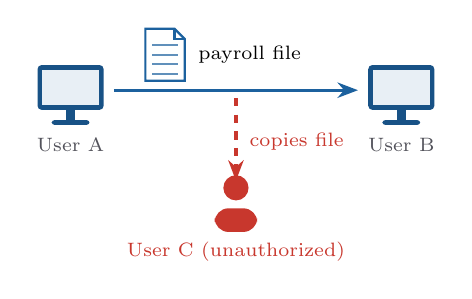
\begin{tikzpicture}
        \pic at (0,0) {pc=ocean}; \node[tag] at (0,-0.5) {User A};
        \pic at (4.2,0) {pc=ocean}; \node[tag] at (4.2,-0.5) {User B};
        \draw[flow=ocean] (0.55,0.2) -- (3.65,0.2);
        \pic at (1.2,0.65) {doc=ocean}; \node[font=\scriptsize,anchor=west] at (1.5,0.65) {payroll file};
        \pic at (2.1,-1.5) {person=brick}; \node[tag,text=brick] at (2.1,-1.85) {User C (unauthorized)};
        \draw[brick,very thick,dashed,->] (2.1,0.1) -- (2.1,-0.95);
        \node[font=\scriptsize,text=brick,right] at (2.15,-0.45) {copies file};
      \end{tikzpicture}
      \par\vspace{1mm}
      {\small C \textbf{monitors} the transmission and \textbf{captures} a copy of sensitive data.}
    \end{column}
    \begin{column}{0.49\textwidth}
      \centering\textbf{\textcolor{grape}{Example 2: Alteration}}\\[2mm]
      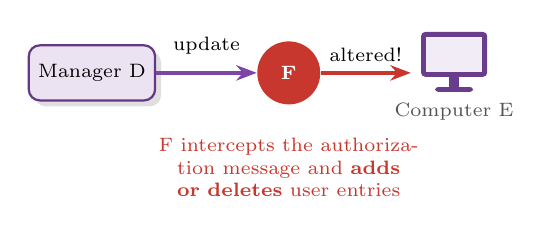
\begin{tikzpicture}
        \node[box=grape,minimum width=14mm,minimum height=7mm,font=\scriptsize] (d) at (-0.4,0) {Manager D};
        \pic at (4.2,0) {pc=grape}; \node[tag] at (4.2,-0.5) {Computer E};
        \node[circle,fill=brick,text=white,font=\scriptsize\bfseries,minimum size=8mm] (f) at (2.1,0) {F};
        \draw[flow=grape] (d) -- node[above=1mm,font=\scriptsize]{update} (f);
        \draw[flow=brick] (f) -- node[above,font=\scriptsize]{altered!} (3.65,0);
        \node[tag,text=brick,text width=4.2cm] at (2.1,-1.2) {F intercepts the authorization message and \textbf{adds or deletes} user entries};
      \end{tikzpicture}
      \par\vspace{1mm}
      {\small A forged \textbf{authorization file} gives access to the wrong people.}
    \end{column}
  \end{columns}
  \vspace{3mm}
  \begin{exampleblock}{Takeaway}
    \small Network security means protocols that let us use the Internet \textbf{comfortably}, without worrying about such attacks.
  \end{exampleblock}
\end{frame}

% ------------------------------------------------------------
\begin{frame}{The Three Security Goals: The CIA Triad}
  \begin{columns}[c]
    \begin{column}{0.5\textwidth}
      \centering
      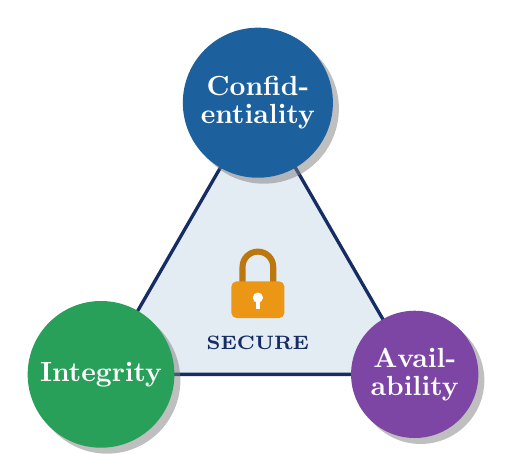
\begin{tikzpicture}
        \coordinate (T) at (90:2.3); \coordinate (L) at (210:2.3); \coordinate (R) at (330:2.3);
        \fill[ocean!12,draw=navy,very thick,rounded corners=6pt] (T) -- (L) -- (R) -- cycle;
        \node[circle,fill=ocean,text=white,font=\bfseries,minimum size=15mm,align=center,drop shadow] at (T) {Confid-\\[-2pt]entiality};
        \node[circle,fill=leaf,text=white,font=\bfseries,minimum size=15mm,drop shadow] at (L) {Integrity};
        \node[circle,fill=grape,text=white,font=\bfseries,minimum size=15mm,align=center,drop shadow] at (R) {Avail-\\[-2pt]ability};
        \pic[scale=1.3] at (0,-0.15) {lock=amber};
        \node[font=\scriptsize\bfseries,text=navy] at (0,-0.75) {SECURE};
      \end{tikzpicture}
    \end{column}
    \begin{column}{0.48\textwidth}
      \begin{itemize}\setlength{\itemsep}{8pt}
        \item[\textcolor{ocean}{\Large\textbullet}] \textbf{Confidentiality}: hide information from \emph{unauthorized access}
        \item[\textcolor{leaf}{\Large\textbullet}] \textbf{Integrity}: protect information from \emph{unauthorized change}
        \item[\textcolor{grape}{\Large\textbullet}] \textbf{Availability}: information is available to \emph{authorized entities when needed}
      \end{itemize}
      \vspace{3mm}
      \begin{block}{Remember}
        \small Every attack threatens at least one of these three goals.
      \end{block}
    \end{column}
  \end{columns}
\end{frame}

% ------------------------------------------------------------
\begin{frame}{The CIA Goals in Everyday Life}
  \centering
  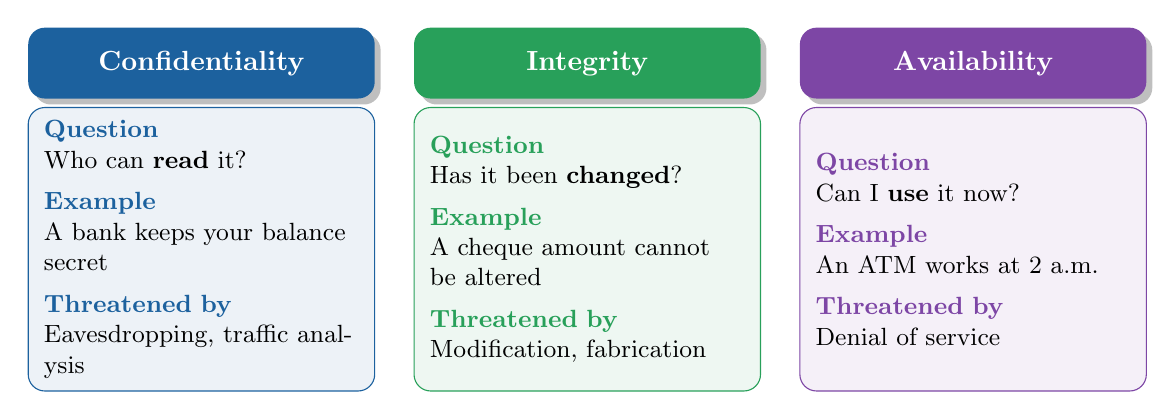
\begin{tikzpicture}
    \foreach \x/\c/\t/\q/\e/\f [count=\k] in {
      0/ocean/Confidentiality/Who can \textbf{read} it?/A bank keeps your balance secret/Eavesdropping\comma{} traffic analysis,
      4.9/leaf/Integrity/Has it been \textbf{changed}?/A cheque amount cannot be altered/Modification\comma{} fabrication,
      9.8/grape/Availability/Can I \textbf{use} it now?/An ATM works at 2 a.m./Denial of service}
    {
      \node[fill=\c,text=white,rounded corners=6pt,minimum width=44mm,minimum height=9mm,font=\bfseries,drop shadow] (h\k) at (\x,0) {\t};
      \node[draw=\c,fill=\c!8,rounded corners=6pt,minimum width=44mm,minimum height=36mm,anchor=north,
        text width=40mm,align=left,font=\small] at ([yshift=-1mm]h\k.south)
        {\textcolor{\c}{\textbf{Question}}\\ \q\\[4pt]
         \textcolor{\c}{\textbf{Example}}\\ \e\\[4pt]
         \textcolor{\c}{\textbf{Threatened by}}\\ \f};
    }
  \end{tikzpicture}
\end{frame}


\begin{frame}{Cryptology = Cryptography + Cryptanalysis}
  \centering
  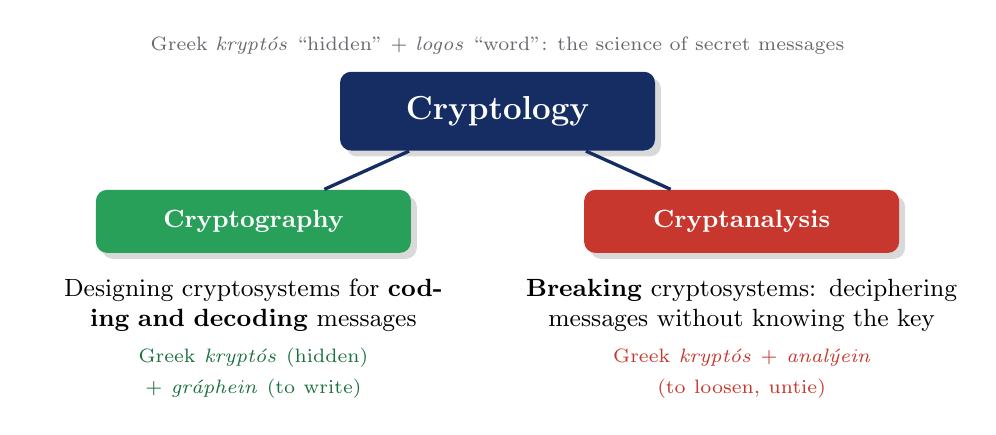
\begin{tikzpicture}[level distance=14mm,
      level 1/.style={sibling distance=62mm},
      edge from parent/.style={draw=navy,very thick}]
    \node[solid box=navy,minimum width=40mm,minimum height=10mm,font=\large\bfseries] {Cryptology}
      child {node[solid box=leaf,minimum width=40mm] (cg) {Cryptography}}
      child {node[solid box=brick,minimum width=40mm] (ca) {Cryptanalysis}};
    \node[tag,above=1mm of cg.north west,anchor=south east] {};
    \node[below=2mm of cg,text width=55mm,align=center,font=\small] {Designing cryptosystems for \textbf{coding and decoding} messages\\[2pt]
      \textcolor{leaf!70!black}{\scriptsize Greek \emph{kryptós} (hidden) + \emph{gráphein} (to write)}};
    \node[below=2mm of ca,text width=55mm,align=center,font=\small] {\textbf{Breaking} cryptosystems: deciphering messages without knowing the key\\[2pt]
      \textcolor{brick}{\scriptsize Greek \emph{kryptós} + \emph{analýein} (to loosen, untie)}};
    \node[above=1mm of current bounding box.north,font=\scriptsize,text=ink!70] {Greek \emph{kryptós} ``hidden'' + \emph{logos} ``word'': the science of secret messages};
  \end{tikzpicture}
  \begin{alertblock}{Common mistake}
    \small Cryptology is often wrongly treated as a synonym for cryptography. It is the \textbf{broader} term that covers both.
  \end{alertblock}
\end{frame}


% ------------------------------------------------------------
\begin{frame}{The Basic Encryption Model}
  \centering
  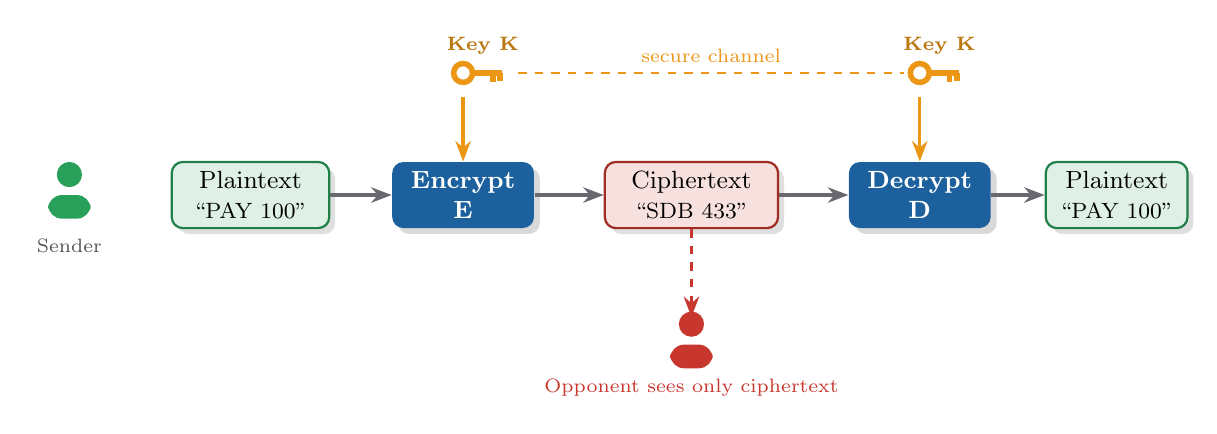
\begin{tikzpicture}[node distance=9mm]
    \pic at (0,0) {person=leaf}; \node[tag] at (0,-0.45) {Sender};
    \node[box=leaf,minimum width=20mm] (pt) at (2.3,0.2) {Plaintext\\\footnotesize ``PAY 100''};
    \node[solid box=ocean,minimum width=18mm] (e) at (5.0,0.2) {Encrypt\\E};
    \node[box=brick,minimum width=22mm] (ct) at (7.9,0.2) {Ciphertext\\\footnotesize ``SDB 433''};
    \node[solid box=ocean,minimum width=18mm] (d) at (10.8,0.2) {Decrypt\\D};
    \node[box=leaf,minimum width=18mm] (pt2) at (13.3,0.2) {Plaintext\\\footnotesize ``PAY 100''};
    \draw[flow] (pt) -- (e); \draw[flow] (e) -- (ct); \draw[flow] (ct) -- (d); \draw[flow] (d) -- (pt2);
    \pic at (5.0,1.75) {key=amber}; \node[font=\scriptsize\bfseries,text=amber!80!black] at (5.25,2.1) {Key K};
    \pic at (10.8,1.75) {key=amber}; \node[font=\scriptsize\bfseries,text=amber!80!black] at (11.05,2.1) {Key K};
    \draw[amber,very thick,->] (5.0,1.45) -- (e.north);
    \draw[amber,very thick,->] (10.8,1.45) -- (d.north);
    \draw[amber,dashed,thick] (5.7,1.75) -- node[above,font=\scriptsize]{secure channel} (10.6,1.75);
    \pic at (7.9,-1.9) {person=brick}; \node[tag,text=brick] at (7.9,-2.25) {Opponent sees only ciphertext};
    \draw[brick,dashed,very thick,->] (ct.south) -- (7.9,-1.35);
  \end{tikzpicture}
  \vspace{2mm}
  \begin{columns}[T]
    \begin{column}{0.5\textwidth}\small
      \textbf{Plaintext}: the original readable message\\
      \textbf{Ciphertext}: the scrambled, unreadable message
    \end{column}
    \begin{column}{0.46\textwidth}\small
      \textbf{Cipher}: the algorithm (E and D)\\
      \textbf{Key}: the secret value that controls the cipher
    \end{column}
  \end{columns}
\end{frame}


\begin{frame}{Three Aspects of Information Security}
  \centering
  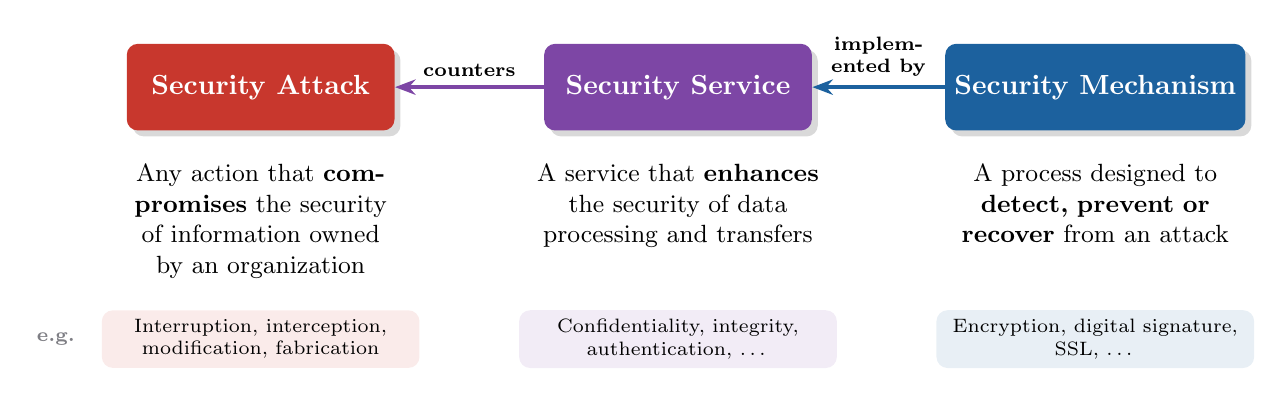
\begin{tikzpicture}
    \node[solid box=brick,minimum width=34mm,minimum height=11mm,font=\bfseries] (a) at (0,0) {Security Attack};
    \node[solid box=grape,minimum width=34mm,minimum height=11mm,font=\bfseries] (s) at (5.3,0) {Security Service};
    \node[solid box=ocean,minimum width=34mm,minimum height=11mm,font=\bfseries] (m) at (10.6,0) {Security Mechanism};
    \draw[flow=grape,<-] (a) -- node[above,font=\scriptsize\bfseries]{counters} (s);
    \draw[flow=ocean,<-] (s) -- node[above,font=\scriptsize\bfseries,align=center]{implem-\\ented by} (m);
    \node[text width=38mm,align=center,font=\small,below=3mm of a] {Any action that \textbf{compromises} the security of information owned by an organization};
    \node[text width=38mm,align=center,font=\small,below=3mm of s] {A service that \textbf{enhances} the security of data processing and transfers};
    \node[text width=38mm,align=center,font=\small,below=3mm of m] {A process designed to \textbf{detect, prevent or recover} from an attack};
    \node[fill=brick!10,rounded corners,text width=38mm,align=center,font=\scriptsize] at (0,-3.2) {Interruption, interception,\\modification, fabrication};
    \node[fill=grape!10,rounded corners,text width=38mm,align=center,font=\scriptsize] at (5.3,-3.2) {Confidentiality, integrity,\\authentication, \dots};
    \node[fill=ocean!10,rounded corners,text width=38mm,align=center,font=\scriptsize] at (10.6,-3.2) {Encryption, digital signature,\\SSL, \dots};
    \node[font=\scriptsize\bfseries,text=ink!60] at (-2.6,-3.2) {e.g.};
  \end{tikzpicture}
  \vspace{2mm}
  \begin{block}{Why these three?}
    \small They help an organization \textbf{identify its security needs} and \textbf{evaluate} security products and policies.
  \end{block}
\end{frame}

% ------------------------------------------------------------
\begin{frame}{An Analogy: Securing a House}
  \centering
  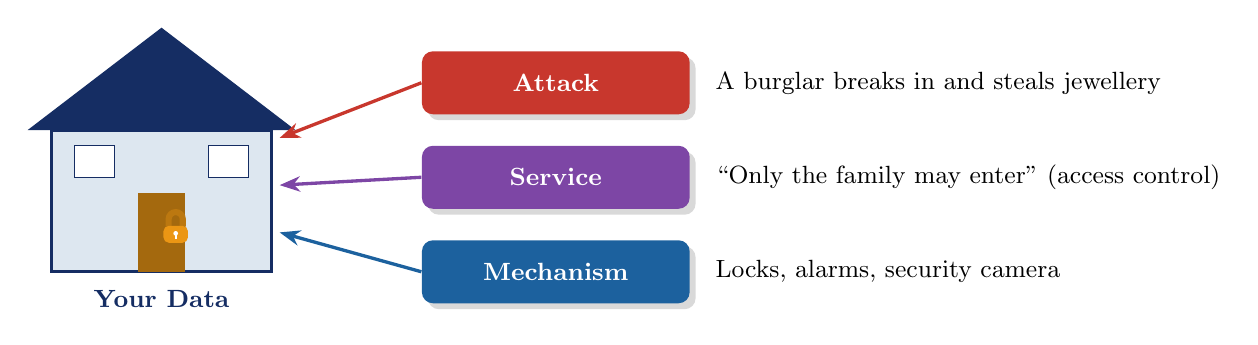
\begin{tikzpicture}
    % house
    \fill[ocean!15,draw=navy,very thick] (-1.4,-1.2) rectangle (1.4,0.6);
    \fill[navy] (-1.7,0.6) -- (0,1.9) -- (1.7,0.6) -- cycle;
    \fill[amber!70!black] (-0.3,-1.2) rectangle (0.3,-0.2);
    \fill[white,draw=navy] (-1.1,0) rectangle (-0.6,0.4);
    \fill[white,draw=navy] (0.6,0) rectangle (1.1,0.4);
    \pic[scale=0.6] at (0.18,-0.7) {lock=amber};
    \node[font=\small\bfseries,text=navy] at (0,-1.55) {Your Data};
    % labels
    \node[solid box=brick,minimum width=34mm,anchor=west] (a) at (3.3,1.2) {Attack};
    \node[anchor=west,font=\small] at ([xshift=2mm]a.east) {A burglar breaks in and steals jewellery};
    \node[solid box=grape,minimum width=34mm,anchor=west] (s) at (3.3,0) {Service};
    \node[anchor=west,font=\small] at ([xshift=2mm]s.east) {``Only the family may enter'' (access control)};
    \node[solid box=ocean,minimum width=34mm,anchor=west] (m) at (3.3,-1.2) {Mechanism};
    \node[anchor=west,font=\small] at ([xshift=2mm]m.east) {Locks, alarms, security camera};
    \draw[brick,very thick,->] (a.west) -- (1.5,0.5);
    \draw[grape,very thick,->] (s.west) -- (1.5,-0.1);
    \draw[ocean,very thick,->] (m.west) -- (1.5,-0.7);
  \end{tikzpicture}
  \vspace{4mm}
  \begin{exampleblock}{Mapping to networks}
    \small Burglar = hacker \quad$\cdot$\quad ``Only family may enter'' = access control / confidentiality service \quad$\cdot$\quad Lock = encryption mechanism
  \end{exampleblock}
\end{frame}

% ------------------------------------------------------------
\begin{frame}{Services Use Mechanisms}
  \centering
  \renewcommand{\arraystretch}{1.12}\small
  \begin{tabular}{>{\columncolor{grape!10}}p{3.2cm} p{5.2cm} >{\columncolor{ocean!8}}p{4.6cm}}
    \toprule
    \rowcolor{navy}\textcolor{white}{\textbf{Security service}} & \textcolor{white}{\textbf{What it guarantees}} & \textcolor{white}{\textbf{Typical mechanism}}\\
    \midrule
    Confidentiality  & Only authorized parties can read data & Encryption \\
    Integrity        & Data is not altered in transit       & Hash / message digest, digital signature \\
    Authentication   & The sender is who they claim to be   & Digital signature, passwords \\
    Non-repudiation  & The sender cannot deny sending       & Digital signature \\
    Access control   & Only permitted users use a resource  & Access-control lists, passwords \\
    Availability     & The service stays usable             & Redundancy, filtering \\
    \bottomrule
  \end{tabular}
  \vspace{2mm}
  \begin{block}{Key point}
    \small A service is \textbf{what} we want; a mechanism is \textbf{how} we get it. One service may use \textbf{one or more} mechanisms.
  \end{block}
\end{frame}


\newcommand{\flowpair}[1][]{%
  \node[station=leaf] (S) at (0,0) {Source};
  \node[station=ocean] (D) at (5,0) {Dest.};
}

\begin{frame}{Normal Flow of Information}
  \begin{columns}[c]
    \begin{column}{0.52\textwidth}
      \centering
      \begin{tikzpicture}
        \flowpair
        \draw[flow=leaf,line width=2pt] (S) -- node[above,font=\small]{message} (D);
        \pic at (2.5,1.05) {doc=leaf};
      \end{tikzpicture}
    \end{column}
    \begin{column}{0.46\textwidth}
      \begin{itemize}\setlength{\itemsep}{6pt}
        \item Information flows from an \good{information source} (a file or a user)\dots
        \item \dots to an \hl{information destination} (another file or user)
        \item Nobody interferes: this is the \textbf{normal} case
      \end{itemize}
      \vspace{2mm}
      \begin{block}{Four general categories of attack}
        \small Each attack below \textbf{changes} this picture in a different way.
      \end{block}
    \end{column}
  \end{columns}
  \vspace{4mm}
  \centering
  
\begin{tikzpicture}
    \foreach \x/\c/\t in {0/brick/Interruption,3.5/amber/Interception,7/grape/Modification,10.5/aqua/Fabrication}
      \node[solid box=\c,minimum width=30mm] at (\x,0) {\t};
  \end{tikzpicture}
\end{frame}

% ------------------------------------------------------------
\begin{frame}{Attack 1: Interruption}
  \begin{columns}[c]
    \begin{column}{0.52\textwidth}
      \centering
      \begin{tikzpicture}
        \flowpair
        \draw[leaf,line width=2pt] (S) -- (2.1,0);
        \draw[brick,line width=3pt] (2.3,-0.55) -- (2.3,0.55);
        \node[brick,font=\Large\bfseries] at (2.75,0) {$\times$};
        \node[tag,text=brick] at (2.4,-0.95) {communication cut};
      \end{tikzpicture}
    \end{column}
    \begin{column}{0.46\textwidth}
      \begin{alertblock}{Definition}
        An asset of the system is \textbf{destroyed} or becomes \textbf{unavailable} or unusable.
      \end{alertblock}
      \vspace{1mm}
      \textbf{Threatens:} \textcolor{grape}{\textbf{Availability}}\\[3pt]
      \textbf{Examples}
      \begin{itemize}\small
        \item Cutting a communication line
        \item Destroying a hard disk
        \item Disabling a file-management system
        \item Flooding a server (\textbf{denial of service})
      \end{itemize}
    \end{column}
  \end{columns}
\end{frame}

% ------------------------------------------------------------
\begin{frame}{Attack 2: Interception}
  \begin{columns}[c]
    \begin{column}{0.52\textwidth}
      \centering
      \begin{tikzpicture}
        \flowpair
        \draw[flow=leaf,line width=2pt] (S) -- (D);
        \node[station=brick] (E) at (2.5,-2.3) {Attacker};
        \draw[flow=brick,dashed,line width=1.5pt] (2.5,0) -- (E);
        \node[tag,text=brick] at (3.4,-1.0) {secret copy};
      \end{tikzpicture}
    \end{column}
    \begin{column}{0.46\textwidth}
      \begin{alertblock}{Definition}
        An \textbf{unauthorized party gains access} to an asset.
      \end{alertblock}
      \vspace{1mm}
      \textbf{Threatens:} \textcolor{ocean}{\textbf{Confidentiality}}\\[3pt]
      \textbf{Examples}
      \begin{itemize}\small
        \item Wiretapping to capture data
        \item Illicit copying of files or programs
        \item Sniffing passwords on a Wi-Fi network
      \end{itemize}
      \vspace{1mm}
      {\small\textcolor{ink!70}{The original message still arrives, so this attack is hard to notice.}}
    \end{column}
  \end{columns}
\end{frame}

% ------------------------------------------------------------
\begin{frame}{Attack 3: Modification}
  \begin{columns}[c]
    \begin{column}{0.52\textwidth}
      \centering
      \begin{tikzpicture}
        \flowpair
        \node[station=brick] (E) at (2.5,-2.3) {Attacker};
        \draw[flow=leaf,line width=2pt] (S) to[out=-20,in=150] (E);
        \draw[flow=brick,line width=2pt] (E) to[out=30,in=200] (D);
        \node[tag,text=leaf!60!black] at (0.6,-1.3) {``Pay 100''};
        \node[tag,text=brick] at (4.4,-1.3) {``Pay 900''};
      \end{tikzpicture}
    \end{column}
    \begin{column}{0.46\textwidth}
      \begin{alertblock}{Definition}
        An unauthorized party not only gains access but also \textbf{tampers} with the asset.
      \end{alertblock}
      \vspace{1mm}
      \textbf{Threatens:} \textcolor{leaf!70!black}{\textbf{Integrity}}\\[3pt]
      \textbf{Examples}
      \begin{itemize}\small
        \item Changing values in a data file
        \item Altering a program so it behaves differently
        \item Modifying the content of a message in transit
      \end{itemize}
    \end{column}
  \end{columns}
\end{frame}

% ------------------------------------------------------------
\begin{frame}{Attack 4: Fabrication}
  \begin{columns}[c]
    \begin{column}{0.52\textwidth}
      \centering
      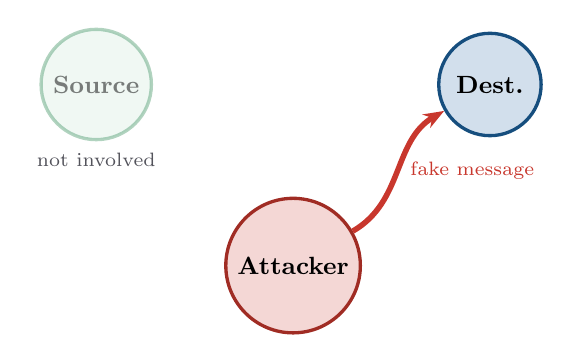
\begin{tikzpicture}
        \node[station=leaf,opacity=0.35,text opacity=0.5] (S) at (0,0) {Source};
        \node[station=ocean] (D) at (5,0) {Dest.};
        \node[station=brick] (E) at (2.5,-2.3) {Attacker};
        \draw[flow=brick,line width=2pt] (E) to[out=30,in=210] node[right,font=\scriptsize,text=brick]{fake message} (D);
        \node[tag] at (0,-0.95) {not involved};
      \end{tikzpicture}
    \end{column}
    \begin{column}{0.46\textwidth}
      \begin{alertblock}{Definition}
        An unauthorized party \textbf{inserts counterfeit objects} into the system.
      \end{alertblock}
      \vspace{1mm}
      \textbf{Threatens:} \textcolor{aqua!70!black}{\textbf{Authenticity}} (integrity of origin)\\[3pt]
      \textbf{Examples}
      \begin{itemize}\small
        \item Inserting spurious messages into a network
        \item Adding a fake record to a file
        \item Phishing e-mail ``from your bank''
      \end{itemize}
    \end{column}
  \end{columns}
\end{frame}

% ------------------------------------------------------------
\begin{frame}{Passive vs. Active Attacks}
  \centering
  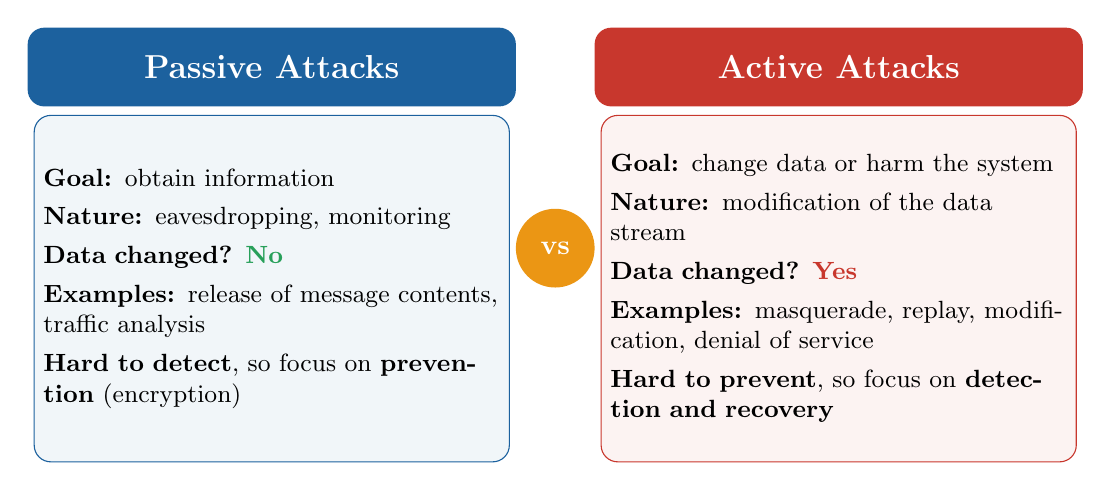
\begin{tikzpicture}
    \node[fill=ocean,text=white,rounded corners=6pt,minimum width=62mm,minimum height=10mm,font=\large\bfseries] (p) at (0,0) {Passive Attacks};
    \node[fill=brick,text=white,rounded corners=6pt,minimum width=62mm,minimum height=10mm,font=\large\bfseries] (a) at (7.2,0) {Active Attacks};
    \node[draw=ocean,fill=ocean!6,rounded corners=6pt,text width=58mm,minimum height=44mm,anchor=north,font=\small] at ([yshift=-1mm]p.south) {
      \textbf{Goal:} obtain information\\[3pt]
      \textbf{Nature:} eavesdropping, monitoring\\[3pt]
      \textbf{Data changed?} \good{No}\\[3pt]
      \textbf{Examples:} release of message contents, traffic analysis\\[3pt]
      \textbf{Hard to detect}, so focus on \textbf{prevention} (encryption)};
    \node[draw=brick,fill=brick!6,rounded corners=6pt,text width=58mm,minimum height=44mm,anchor=north,font=\small] at ([yshift=-1mm]a.south) {
      \textbf{Goal:} change data or harm the system\\[3pt]
      \textbf{Nature:} modification of the data stream\\[3pt]
      \textbf{Data changed?} \bad{Yes}\\[3pt]
      \textbf{Examples:} masquerade, replay, modification, denial of service\\[3pt]
      \textbf{Hard to prevent}, so focus on \textbf{detection and recovery}};
    \node[circle,fill=amber,text=white,font=\bfseries,minimum size=10mm] at (3.6,-2.3) {vs};
  \end{tikzpicture}
\end{frame}



\begin{frame}{Model of a Conventional Cryptosystem}
  \centering
  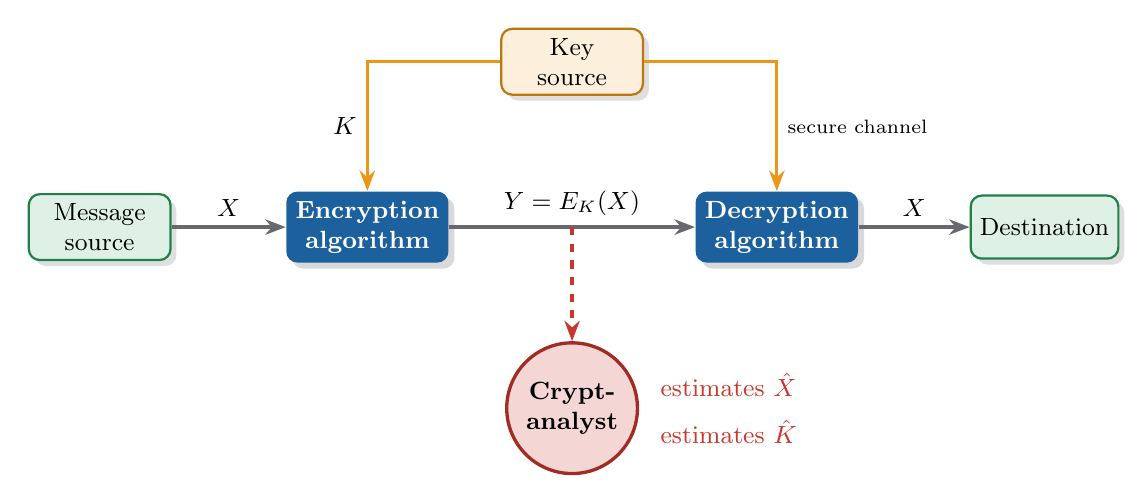
\begin{tikzpicture}
    \node[box=leaf,minimum width=18mm] (src) at (0,0) {Message\\source};
    \node[solid box=ocean,minimum width=20mm] (enc) at (3.4,0) {Encryption\\algorithm};
    \node[solid box=ocean,minimum width=20mm] (dec) at (8.6,0) {Decryption\\algorithm};
    \node[box=leaf,minimum width=18mm] (dst) at (12,0) {Destination};
    \node[box=amber,minimum width=18mm] (ks) at (6,2.1) {Key\\source};
    \draw[flow] (src) -- node[above,font=\small]{$X$} (enc);
    \draw[flow] (enc) -- node[above,font=\small]{$Y = E_K(X)$} (dec);
    \draw[flow] (dec) -- node[above,font=\small]{$X$} (dst);
    \draw[flow=amber] (ks) -| node[pos=0.75,left,font=\small]{$K$} (enc);
    \draw[flow=amber] (ks) -| node[pos=0.75,right,font=\scriptsize]{secure channel} (dec);
    \node[station=brick,minimum size=16mm] (cr) at (6,-2.3) {Crypt-\\analyst};
    \draw[flow=brick,dashed] (6,0) -- (cr);
    \node[anchor=west,font=\small,text=brick] at (7,-2.0) {estimates $\hat{X}$};
    \node[anchor=west,font=\small,text=brick] at (7,-2.6) {estimates $\hat{K}$};
  \end{tikzpicture}
  \vspace{2mm}
  \begin{itemize}\small
    \item The opponent sees \textbf{$Y$} but not $K$ or $X$, and is assumed to \textbf{know the algorithms} E and D
    \item Recovering $\hat{X}$ breaks \textbf{one message}; recovering $\hat{K}$ breaks \bad{all past and future messages}
  \end{itemize}
\end{frame}

% ------------------------------------------------------------
\begin{frame}{Three Dimensions of Cryptographic Systems}
  \centering
  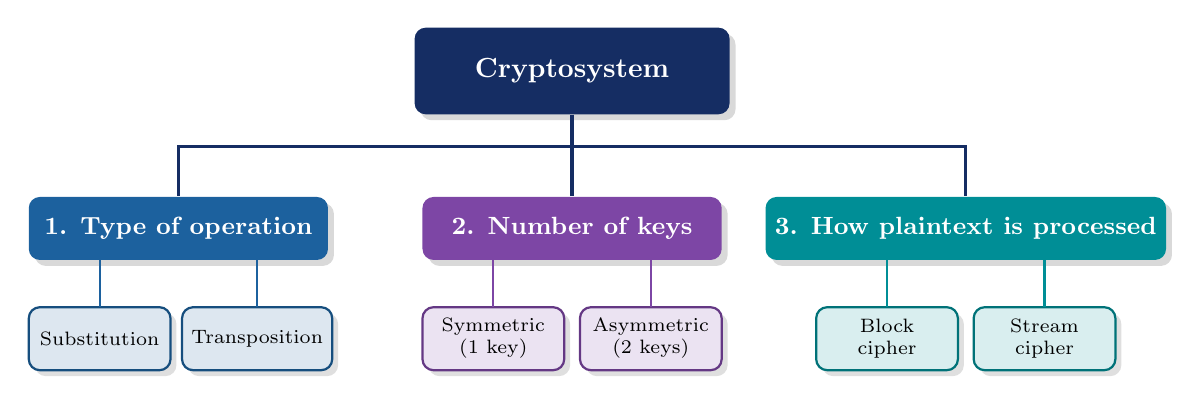
\begin{tikzpicture}
    \node[solid box=navy,minimum width=40mm,minimum height=11mm,font=\bfseries] (c) at (0,0) {Cryptosystem};
    \node[solid box=ocean,minimum width=38mm] (d1) at (-5,-2) {1. Type of operation};
    \node[solid box=grape,minimum width=38mm] (d2) at (0,-2) {2. Number of keys};
    \node[solid box=aqua,minimum width=38mm] (d3) at (5,-2) {3. How plaintext is processed};
    \foreach \n in {d1,d2,d3} \draw[navy,very thick] (c.south) -- ++(0,-0.4) -| (\n.north);
    \node[box=ocean,minimum width=18mm,font=\scriptsize] at (-6,-3.4) {Substitution};
    \node[box=ocean,minimum width=18mm,font=\scriptsize] at (-4,-3.4) {Transposition};
    \node[box=grape,minimum width=18mm,font=\scriptsize] at (-1,-3.4) {Symmetric\\(1 key)};
    \node[box=grape,minimum width=18mm,font=\scriptsize] at (1,-3.4) {Asymmetric\\(2 keys)};
    \node[box=aqua,minimum width=18mm,font=\scriptsize] at (4,-3.4) {Block\\cipher};
    \node[box=aqua,minimum width=18mm,font=\scriptsize] at (6,-3.4) {Stream\\cipher};
    \foreach \x/\c in {-6/ocean,-4/ocean,-1/grape,1/grape,4/aqua,6/aqua} \draw[\c,thick] (\x,-2.4) -- (\x,-3.0);
  \end{tikzpicture}
  \vspace{3mm}
  \begin{block}{Golden rule}
    \small Every operation must be \textbf{reversible}: no information may be lost. Most real systems (\emph{product systems}) combine \textbf{many stages} of substitution and transposition.
  \end{block}
\end{frame}

% ------------------------------------------------------------
\begin{frame}{Dimension 1a: Substitution}
  \begin{columns}[c]
    \begin{column}{0.55\textwidth}
      \centering
      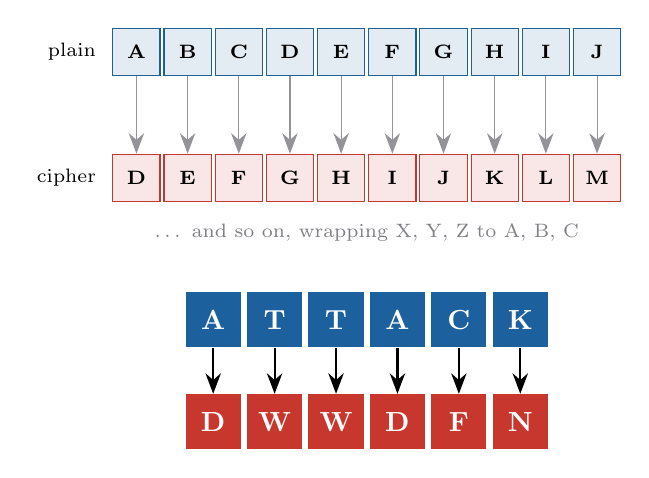
\begin{tikzpicture}[x=6.5mm]
        \foreach \l [count=\i from 0] in {A,B,C,D,E,F,G,H,I,J,K,L,M,N,O,P,Q,R,S,T,U,V,W,X,Y,Z}{
          \ifnum\i<10
            \node[draw=ocean,fill=ocean!12,minimum size=6mm,font=\scriptsize\bfseries] (p\i) at (\i,0) {\l};
          \fi
        }
        \foreach \l [count=\i from 0] in {D,E,F,G,H,I,J,K,L,M}
          \node[draw=brick,fill=brick!12,minimum size=6mm,font=\scriptsize\bfseries] (c\i) at (\i,-1.6) {\l};
        \foreach \i in {0,...,9} \draw[->,ink!50] (p\i) -- (c\i);
        \node[anchor=east,font=\scriptsize] at (-0.6,0) {plain};
        \node[anchor=east,font=\scriptsize] at (-0.6,-1.6) {cipher};
        \node[font=\scriptsize,text=ink!60] at (4.5,-2.3) {\dots\ and so on, wrapping X, Y, Z to A, B, C};
        % example
        \foreach \l [count=\i from 0] in {A,T,T,A,C,K}
          \node[fill=ocean,text=white,minimum size=7mm,font=\bfseries] (x\i) at (\i*1.2+1.5,-3.4) {\l};
        \foreach \l [count=\i from 0] in {D,W,W,D,F,N}{
          \node[fill=brick,text=white,minimum size=7mm,font=\bfseries] (y\i) at (\i*1.2+1.5,-4.7) {\l};
          \draw[->,thick] (x\i) -- (y\i);}
      \end{tikzpicture}
    \end{column}
    \begin{column}{0.43\textwidth}
      \begin{block}{Substitution}
        Each element (bit, letter, group of letters) is \textbf{mapped to another element}.
      \end{block}
      \vspace{2mm}
      \textbf{Example: Caesar cipher (shift 3)}
      \begin{itemize}\small
        \item Each letter moves 3 places forward
        \item \texttt{ATTACK} $\rightarrow$ \texttt{DWWDFN}
        \item Letters \textbf{change}, positions \textbf{stay}
      \end{itemize}
      \vspace{2mm}
      \begin{alertblock}{Weakness}
        \small Only 25 possible shifts, so it is easily broken by trying them all.
      \end{alertblock}
    \end{column}
  \end{columns}
\end{frame}

% ------------------------------------------------------------
\begin{frame}{Dimension 1b: Transposition}
  \begin{columns}[c]
    \begin{column}{0.55\textwidth}
      \centering
      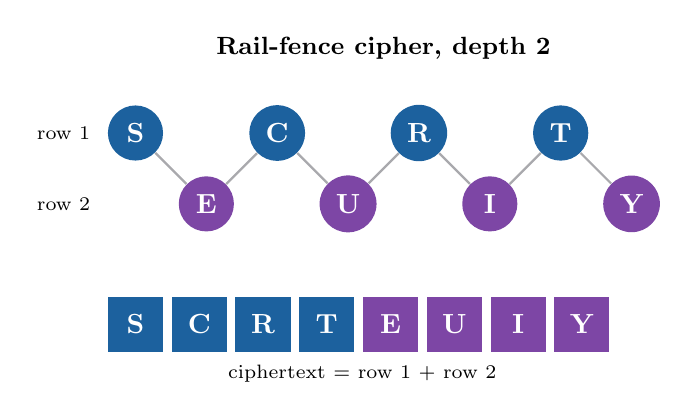
\begin{tikzpicture}[x=9mm,y=9mm]
        \node[font=\small\bfseries] at (3.5,1.2) {Rail-fence cipher, depth 2};
        \foreach \l [count=\i from 0] in {S,E,C,U,R,I,T,Y}{
          \pgfmathsetmacro{\row}{mod(\i,2)==0 ? 0 : -1}
          \pgfmathtruncatemacro{\ev}{mod(\i,2)}
          \ifnum\ev=0
            \node[circle,fill=ocean,text=white,font=\bfseries,minimum size=7mm] (r\i) at (\i,\row) {\l};
          \else
            \node[circle,fill=grape,text=white,font=\bfseries,minimum size=7mm] (r\i) at (\i,\row) {\l};
          \fi
        }
        \foreach \i [evaluate=\i as \j using int(\i+1)] in {0,...,6} \draw[ink!40,thick] (r\i) -- (r\j);
        \node[anchor=east,font=\scriptsize] at (-0.5,0) {row 1};
        \node[anchor=east,font=\scriptsize] at (-0.5,-1) {row 2};
        \foreach \l [count=\i from 0] in {S,C,R,T}
          \node[fill=ocean,text=white,minimum size=7mm,font=\bfseries] at (\i*0.9,-2.7) {\l};
        \foreach \l [count=\i from 4] in {E,U,I,Y}
          \node[fill=grape,text=white,minimum size=7mm,font=\bfseries] at (\i*0.9,-2.7) {\l};
        \node[font=\scriptsize] at (3.2,-3.4) {ciphertext = row 1 + row 2};
      \end{tikzpicture}
    \end{column}
    \begin{column}{0.43\textwidth}
      \begin{block}{Transposition}
        Elements of the plaintext are \textbf{rearranged}: same letters, \textbf{new order}.
      \end{block}
      \vspace{2mm}
      \textbf{Example}
      \begin{itemize}\small
        \item Write \texttt{SECURITY} in zig-zag on 2 rows
        \item Read row by row
        \item \texttt{SECURITY} $\rightarrow$ \texttt{SCRTEUIY}
      \end{itemize}
      \vspace{2mm}
      \begin{exampleblock}{Combine both!}
        \small Modern ciphers alternate substitution \emph{and} transposition in many rounds.
      \end{exampleblock}
    \end{column}
  \end{columns}
\end{frame}

% ------------------------------------------------------------
\begin{frame}{Dimension 2: Number of Keys}
  \begin{columns}[T]
    \begin{column}{0.49\textwidth}
      \centering\textbf{\textcolor{ocean}{Symmetric (single-key, secret-key)}}\\[3mm]
      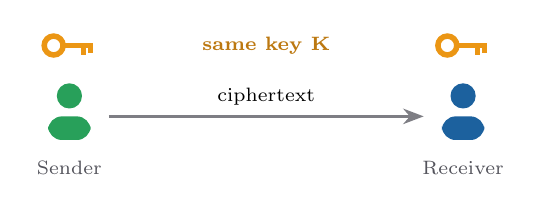
\begin{tikzpicture}
        \pic at (0,0) {person=leaf}; \node[tag] at (0,-0.45) {Sender};
        \pic at (5,0) {person=ocean}; \node[tag] at (5,-0.45) {Receiver};
        \draw[flow=ink!60] (0.5,0.2) -- node[above,font=\scriptsize]{ciphertext} (4.5,0.2);
        \pic at (-0.2,1.1) {key=amber}; \pic at (4.8,1.1) {key=amber};
        \node[font=\scriptsize\bfseries,text=amber!80!black] at (2.5,1.1) {same key K};
      \end{tikzpicture}\\[2mm]
      {\small Also called \textbf{conventional} encryption. Fast, but the key must be \textbf{shared secretly} first.}
    \end{column}
    \begin{column}{0.49\textwidth}
      \centering\textbf{\textcolor{grape}{Asymmetric (two-key, public-key)}}\\[3mm]
      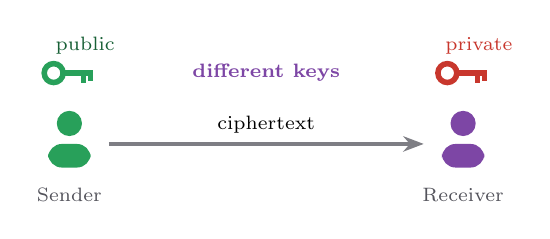
\begin{tikzpicture}
        \pic at (0,0) {person=leaf}; \node[tag] at (0,-0.45) {Sender};
        \pic at (5,0) {person=grape}; \node[tag] at (5,-0.45) {Receiver};
        \draw[flow=ink!60] (0.5,0.2) -- node[above,font=\scriptsize]{ciphertext} (4.5,0.2);
        \pic at (-0.2,1.1) {key=leaf}; \node[font=\scriptsize,text=leaf!60!black] at (0.2,1.45) {public};
        \pic at (4.8,1.1) {key=brick}; \node[font=\scriptsize,text=brick] at (5.2,1.45) {private};
        \node[font=\scriptsize\bfseries,text=grape] at (2.5,1.1) {different keys};
      \end{tikzpicture}\\[2mm]
      {\small Encrypt with the receiver's \textbf{public} key; only their \textbf{private} key decrypts. No secret key to share.}
    \end{column}
  \end{columns}
  \vspace{4mm}
  \begin{block}{Coming later in the course}
    \small Symmetric: DES, IDEA, AES (Modules 6--7) \quad$\cdot$\quad Asymmetric: RSA, Diffie--Hellman, ECC (Module 8)
  \end{block}
\end{frame}

% ------------------------------------------------------------
\begin{frame}{Dimension 3: Block vs. Stream Ciphers}
  \begin{columns}[T]
    \begin{column}{0.49\textwidth}
      \centering\textbf{\textcolor{aqua!70!black}{Block cipher}}\\[3mm]
      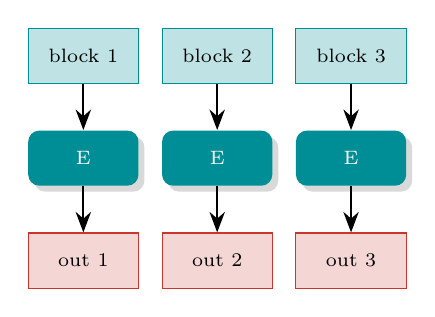
\begin{tikzpicture}
        \foreach \i in {0,1,2} {
          \node[fill=aqua!25,draw=aqua,minimum width=14mm,minimum height=7mm,font=\scriptsize] (in\i) at (\i*1.7,0) {block \the\numexpr\i+1\relax};
          \node[solid box=aqua,minimum width=14mm,minimum height=7mm,font=\scriptsize] (e\i) at (\i*1.7,-1.3) {E};
          \node[fill=brick!20,draw=brick,minimum width=14mm,minimum height=7mm,font=\scriptsize] (o\i) at (\i*1.7,-2.6) {out \the\numexpr\i+1\relax};
          \draw[->,thick] (in\i) -- (e\i); \draw[->,thick] (e\i) -- (o\i);
        }
      \end{tikzpicture}\\[2mm]
      {\small Processes the input \textbf{one block at a time} (e.g. 64 or 128 bits), producing one output block per input block.}
    \end{column}
    \begin{column}{0.49\textwidth}
      \centering\textbf{\textcolor{grape}{Stream cipher}}\\[3mm]
      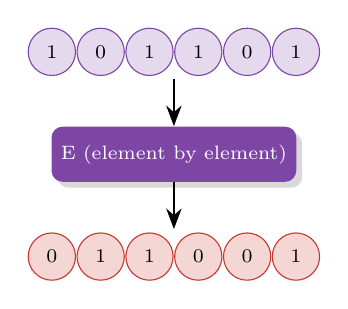
\begin{tikzpicture}
        \foreach \b [count=\i from 0] in {1,0,1,1,0,1}
          \node[circle,fill=grape!20,draw=grape,minimum size=6mm,font=\scriptsize] at (\i*0.62,0) {\b};
        \node[solid box=grape,minimum width=30mm,minimum height=7mm,font=\scriptsize] (e) at (1.55,-1.3) {E (element by element)};
        \foreach \b [count=\i from 0] in {0,1,1,0,0,1}
          \node[circle,fill=brick!20,draw=brick,minimum size=6mm,font=\scriptsize] at (\i*0.62,-2.6) {\b};
        \draw[->,thick] (1.55,-0.35) -- (e); \draw[->,thick] (e) -- (1.55,-2.25);
      \end{tikzpicture}\\[2mm]
      {\small Processes input elements \textbf{continuously}, producing output \textbf{one element at a time} as it goes along.}
    \end{column}
  \end{columns}
  \vspace{1mm}
  \begin{exampleblock}{Analogy}
    \small Block = sealing letters in envelopes one by one \quad$\cdot$\quad Stream = water through a filter, drop by drop
  \end{exampleblock}
\end{frame}


\begin{frame}{Two Ways to Attack a Cryptosystem}
  \centering
  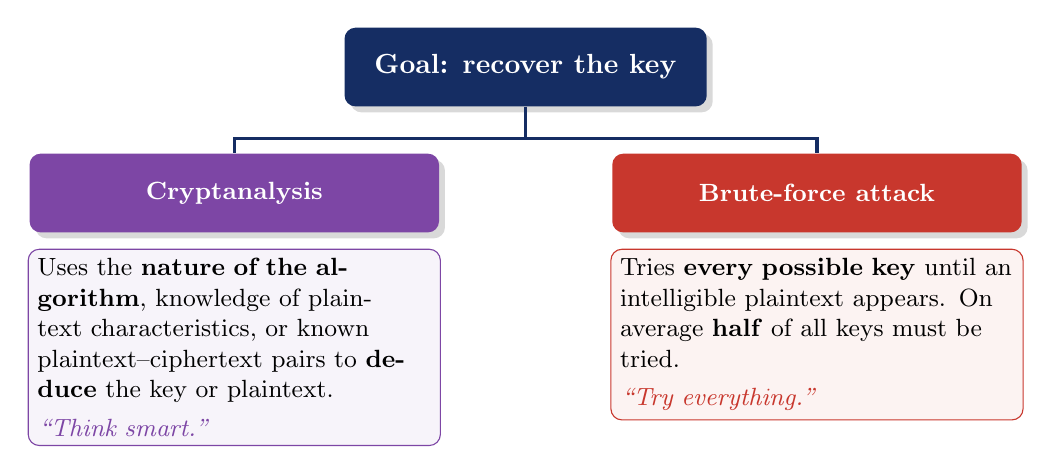
\begin{tikzpicture}
    \node[solid box=navy,minimum width=46mm,minimum height=10mm,font=\bfseries] (g) at (0,0) {Goal: recover the \textbf{key}};
    \node[solid box=grape,minimum width=52mm,minimum height=10mm] (c) at (-3.7,-1.6) {Cryptanalysis};
    \node[solid box=brick,minimum width=52mm,minimum height=10mm] (b) at (3.7,-1.6) {Brute-force attack};
    \draw[navy,very thick] (g.south) -- ++(0,-0.4) -| (c.north);
    \draw[navy,very thick] (g.south) -- ++(0,-0.4) -| (b.north);
    \node[draw=grape,fill=grape!6,rounded corners,text width=50mm,font=\small,anchor=north] at ([yshift=-2mm]c.south)
      {Uses the \textbf{nature of the algorithm}, knowledge of plaintext characteristics, or known plaintext--ciphertext pairs to \textbf{deduce} the key or plaintext.\\[3pt]
       \textcolor{grape}{\textit{``Think smart.''}}};
    \node[draw=brick,fill=brick!6,rounded corners,text width=50mm,font=\small,anchor=north] at ([yshift=-2mm]b.south)
      {Tries \textbf{every possible key} until an intelligible plaintext appears. On average \textbf{half} of all keys must be tried.\\[3pt]
       \textcolor{brick}{\textit{``Try everything.''}}};
  \end{tikzpicture}
  \vspace{1mm}
  \begin{alertblock}{If either succeeds\dots}
    \small \dots \textbf{all future and past messages} encrypted with that key are compromised.
  \end{alertblock}
\end{frame}

% ------------------------------------------------------------
\begin{frame}{Brute Force: Why Key Length Matters}
  \begin{columns}[c]
    \begin{column}{0.53\textwidth}
      \renewcommand{\arraystretch}{1.3}
      \footnotesize
      \begin{tabular}{c c r r}
        \toprule
        \rowcolor{navy}\textcolor{white}{\textbf{Key}} & \textcolor{white}{\textbf{Keys}} & \textcolor{white}{\textbf{@ $10^6$/s}} & \textcolor{white}{\textbf{@ $10^{12}$/s}}\\
        \midrule
        32 bits  & $4.3\times10^{9}$  & 35.8 min & 2.15 ms\\
        56 bits  & $7.2\times10^{16}$ & 1142 years & 10 hours\\
        128 bits & $3.4\times10^{38}$ & $5.4\times10^{24}$ yrs & $5.4\times10^{18}$ yrs\\
        168 bits & $3.7\times10^{50}$ & $5.9\times10^{36}$ yrs & $5.9\times10^{30}$ yrs\\
        \bottomrule
      \end{tabular}\\[2mm]
      {\scriptsize Average time = trying half the key space.}
    \end{column}
    \begin{column}{0.45\textwidth}
      \centering
      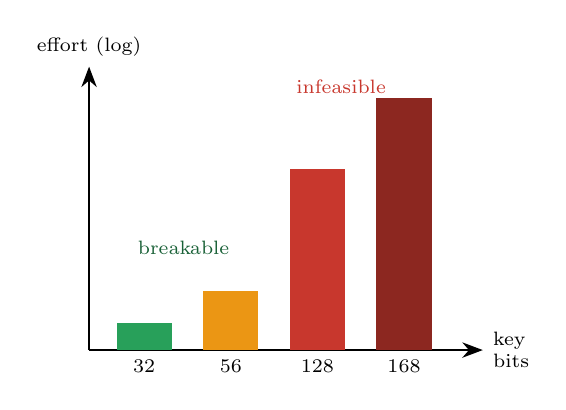
\begin{tikzpicture}
        \draw[->,thick] (0,0) -- (5,0) node[right,font=\scriptsize,align=left]{key\\bits};
        \draw[->,thick] (0,0) -- (0,3.6) node[above,font=\scriptsize]{effort (log)};
        \foreach \x/\h/\l/\c in {0.7/0.35/32/leaf,1.8/0.75/56/amber,2.9/2.3/128/brick,4.0/3.2/168/brick!70!black}{
          \fill[\c] (\x-0.35,0) rectangle (\x+0.35,\h);
          \node[font=\scriptsize,below] at (\x,0) {\l};
        }
        \node[font=\scriptsize,text=leaf!60!black] at (1.2,1.3) {breakable};
        \node[font=\scriptsize,text=brick,align=center] at (3.2,3.35) {infeasible};
      \end{tikzpicture}
    \end{column}
  \end{columns}
  \vspace{3mm}
  \begin{block}{Lesson}
    \small Each extra bit \textbf{doubles} the work. A 128-bit key makes brute force hopeless, so attackers turn to \textbf{cryptanalysis}.
  \end{block}
\end{frame}

% ------------------------------------------------------------
\begin{frame}{Types of Cryptanalytic Attacks}
  \centering
  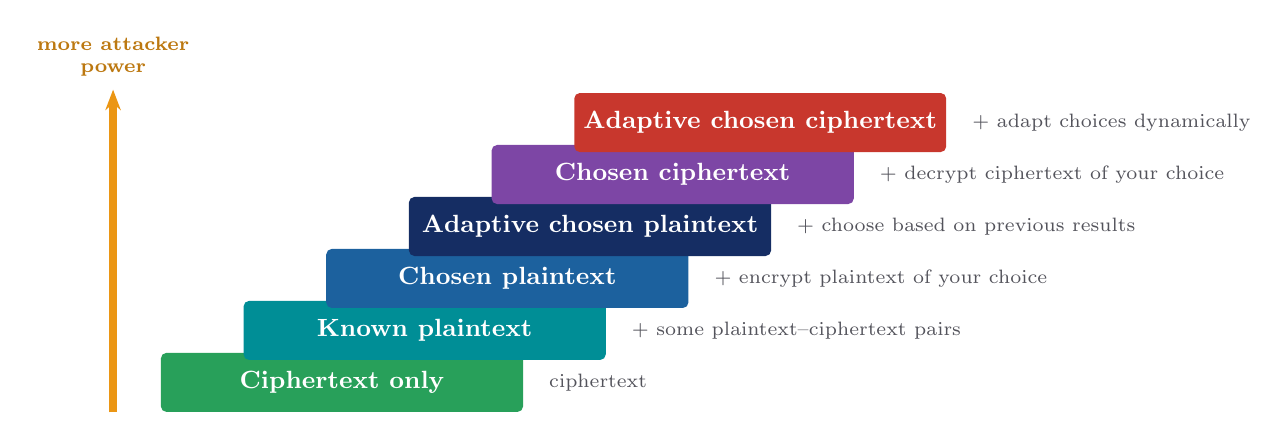
\begin{tikzpicture}
    \foreach \t/\c/\d [count=\i from 0] in {
      Ciphertext only/leaf/ciphertext,
      Known plaintext/aqua/+ some plaintext--ciphertext pairs,
      Chosen plaintext/ocean/+ encrypt plaintext of your choice,
      Adaptive chosen plaintext/navy/+ choose based on previous results,
      Chosen ciphertext/grape/+ decrypt ciphertext of your choice,
      Adaptive chosen ciphertext/brick/+ adapt choices dynamically}
    {
      \node[fill=\c,text=white,font=\small\bfseries,minimum width=46mm,minimum height=7.5mm,anchor=south west,rounded corners=2pt]
        (s\i) at (\i*1.05,\i*0.66) {\t};
      \node[anchor=west,font=\scriptsize,text=ink!80] at ([xshift=2mm]s\i.east) {\d};
    }
    \draw[->,line width=3pt,amber] (-0.6,0) -- (-0.6,4.1) node[above,font=\scriptsize\bfseries,text=amber!80!black,align=center] {more attacker\\power};
  \end{tikzpicture}\par\vspace{1mm}
  {\small The cryptanalyst's strategy depends on \textbf{how much information is available}. Going up the stairs, the attacker knows more and the attack gets easier.}
\end{frame}

% ------------------------------------------------------------
\begin{frame}{Ciphertext-Only and Known-Plaintext Attacks}
  \begin{columns}[T]
    \begin{column}{0.49\textwidth}
      \begin{block}{Ciphertext only}
        \small The cryptanalyst has only a \textbf{sample of ciphertext}, without the plaintext.
      \end{block}
      \centering
      
\begin{tikzpicture}
        \pic at (0,0) {person=brick};
        \node[fill=brick!15,draw=brick,rounded corners,font=\scriptsize\ttfamily] (c) at (2.4,0.2) {XQJZ KPLW};
        \draw[<-,thick,brick] (0.4,0.2) -- (c);
        \node[font=\large\bfseries,text=ink!50] at (4,0.2) {?};
      \end{tikzpicture}\\[1mm]
      \begin{itemize}\scriptsize
        \item Data is \good{easy to obtain}
        \item Attack is \bad{hard}: needs a very large sample
      \end{itemize}
    \end{column}
    \begin{column}{0.49\textwidth}
      \begin{block}{Known plaintext}
        \small The cryptanalyst has a sample of ciphertext \textbf{and the corresponding plaintext}.
      \end{block}
      \centering
      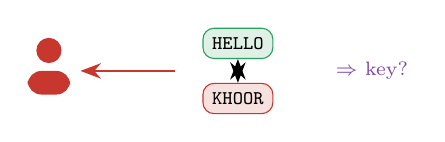
\begin{tikzpicture}
        \pic at (0,0) {person=brick};
        \node[fill=leaf!15,draw=leaf,rounded corners,font=\scriptsize\ttfamily] (p) at (2.4,0.55) {HELLO};
        \node[fill=brick!15,draw=brick,rounded corners,font=\scriptsize\ttfamily] (c) at (2.4,-0.15) {KHOOR};
        \draw[<->,thick] (p) -- (c);
        \draw[<-,thick,brick] (0.4,0.2) -- (1.6,0.2);
        \node[font=\scriptsize,text=grape] at (4.1,0.2) {$\Rightarrow$ key?};
      \end{tikzpicture}\\[1mm]
      \begin{itemize}\scriptsize
        \item E.g. standard headers like ``Dear Sir''
        \item Pairs reveal \textbf{patterns} in the key
      \end{itemize}
    \end{column}
  \end{columns}
\end{frame}

% ------------------------------------------------------------
\begin{frame}{Chosen-Plaintext and Chosen-Ciphertext Attacks}
  \begin{columns}[T]
    \begin{column}{0.49\textwidth}
      \centering
      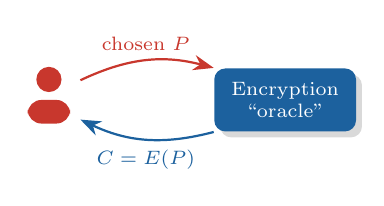
\begin{tikzpicture}
        \pic at (0,0) {person=brick};
        \node[solid box=ocean,minimum width=18mm,font=\scriptsize] (o) at (3,0.2) {Encryption\\``oracle''};
        \draw[->,thick,brick] (0.4,0.45) to[bend left=20] node[above,font=\scriptsize]{chosen $P$} (o.north west);
        \draw[->,thick,ocean] (o.south west) to[bend left=20] node[below,font=\scriptsize]{$C = E(P)$} (0.4,-0.05);
      \end{tikzpicture}
      \begin{block}{Chosen plaintext}
        \small The attacker \textbf{chooses} plaintext and obtains its ciphertext.\\
        \textbf{Adaptive:} choices change \emph{dynamically} based on earlier results.
      \end{block}
    \end{column}
    \begin{column}{0.49\textwidth}
      \centering
      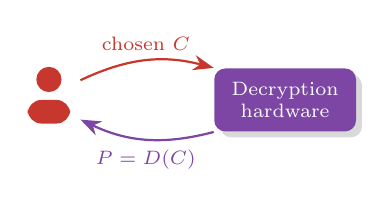
\begin{tikzpicture}
        \pic at (0,0) {person=brick};
        \node[solid box=grape,minimum width=18mm,font=\scriptsize] (o) at (3,0.2) {Decryption\\hardware};
        \draw[->,thick,brick] (0.4,0.45) to[bend left=20] node[above,font=\scriptsize]{chosen $C$} (o.north west);
        \draw[->,thick,grape] (o.south west) to[bend left=20] node[below,font=\scriptsize]{$P = D(C)$} (0.4,-0.05);
      \end{tikzpicture}
      \begin{block}{Chosen ciphertext}
        \small The attacker chooses ciphertext and obtains the decrypted plaintext. Mostly used against \textbf{public-key} systems.\\
        \textbf{Adaptive:} free use of decryption hardware, but cannot extract the key directly.
      \end{block}
    \end{column}
  \end{columns}
\end{frame}


% ============================================================
\section{Network Models}
% ============================================================

\begin{frame}{Why Networks? Data Communication}
  \centering
  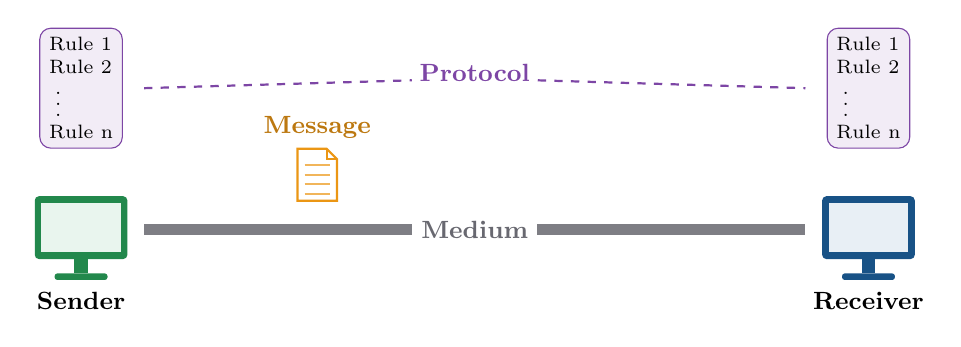
\begin{tikzpicture}
    \pic[scale=1.4] at (0,0) {pc=leaf}; \node[font=\small\bfseries] at (0,-0.6) {Sender};
    \pic[scale=1.4] at (10,0) {pc=ocean}; \node[font=\small\bfseries] at (10,-0.6) {Receiver};
    \draw[ink!60,line width=4pt] (0.8,0.3) -- (9.2,0.3);
    \node[fill=white,font=\small\bfseries,text=ink!70] at (5,0.3) {Medium};
    \pic at (3,1.0) {doc=amber}; \node[font=\small\bfseries,text=amber!80!black] at (3,1.6) {Message};
    \foreach \x in {0,10}{
      \node[draw=grape,fill=grape!10,rounded corners,font=\scriptsize,align=left] at (\x,2.1) {Rule 1\\Rule 2\\\;\vdots\\Rule n};
    }
    \node[font=\small\bfseries,text=grape] at (5,2.3) {Protocol};
    \draw[grape,thick,dashed] (0.8,2.1) -- (4.2,2.2); \draw[grape,thick,dashed] (5.8,2.2) -- (9.2,2.1);
  \end{tikzpicture}
  \vspace{3mm}
  \begin{itemize}\small
    \item Data communication means conveying a message, an idea, a picture or speech that is \textbf{received and understood correctly}
    \item The telephone is instant, but \textbf{pictures and large data} cannot be sent reliably or remembered
    \item So sending data over \textbf{wired and wireless networks} (messages, pictures, voice) has become vital
  \end{itemize}
\end{frame}

% ------------------------------------------------------------
\begin{frame}{Categories of Networks}
  \begin{columns}[c]
    \begin{column}{0.55\textwidth}
      \centering
      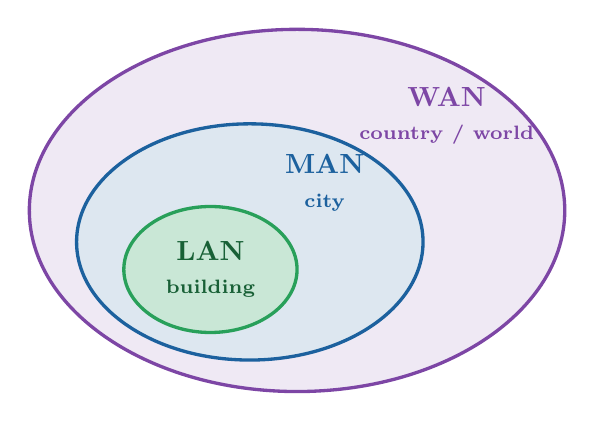
\begin{tikzpicture}
        \fill[grape!12,draw=grape,very thick] (0,0) ellipse (3.4cm and 2.3cm);
        \fill[ocean!15,draw=ocean,very thick] (-0.6,-0.4) ellipse (2.2cm and 1.5cm);
        \fill[leaf!25,draw=leaf,very thick] (-1.1,-0.75) ellipse (1.1cm and 0.8cm);
        \node[font=\bfseries,text=leaf!60!black,align=center] at (-1.1,-0.75) {LAN\\\scriptsize building};
        \node[font=\bfseries,text=ocean,align=center] at (0.35,0.35) {MAN\\\scriptsize city};
        \node[font=\bfseries,text=grape,align=center] at (1.9,1.2) {WAN\\\scriptsize country / world};
      \end{tikzpicture}
    \end{column}
    \begin{column}{0.43\textwidth}
      Three primary categories:
      \begin{itemize}\setlength{\itemsep}{4pt}
        \item \good{Local Area Network (LAN)}
        \item \hl{Metropolitan Area Network (MAN)}
        \item \textcolor{grape}{\textbf{Wide Area Network (WAN)}}
      \end{itemize}
      \vspace{2mm}
      \begin{block}{Category is decided by}
        \small size \,$\cdot$\, ownership \,$\cdot$\, distance covered \,$\cdot$\, physical architecture
      \end{block}
    \end{column}
  \end{columns}
\end{frame}

% ------------------------------------------------------------
\begin{frame}{Local Area Network (LAN)}
  \centering
  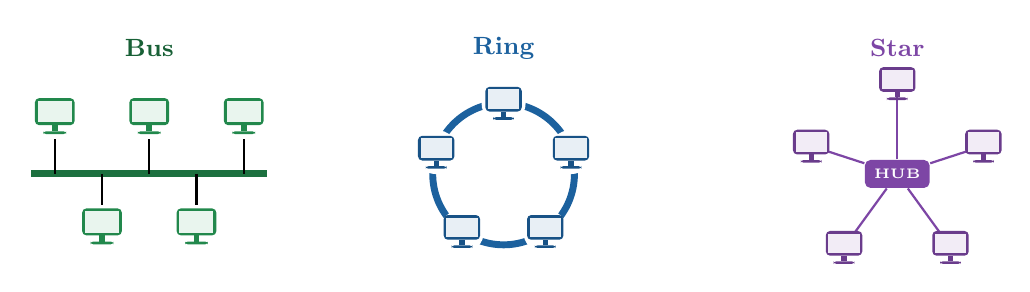
\begin{tikzpicture}
    % Bus
    \begin{scope}[shift={(0,0)}]
      \node[font=\small\bfseries,text=leaf!60!black] at (1.5,1.6) {Bus};
      \draw[leaf!70!black,line width=2.5pt] (0,0) -- (3,0);
      \foreach \x in {0.3,1.5,2.7}{ \draw[thick] (\x,0) -- (\x,0.45); \pic[scale=0.6] at (\x,0.65) {pc=leaf}; }
      \foreach \x in {0.9,2.1}{ \draw[thick] (\x,0) -- (\x,-0.4); \pic[scale=0.6] at (\x,-0.75) {pc=leaf}; }
    \end{scope}
    % Ring
    \begin{scope}[shift={(6,0)}]
      \node[font=\small\bfseries,text=ocean] at (0,1.6) {Ring};
      \draw[ocean,line width=2.5pt] (0,0) circle (0.9);
      \foreach \a in {90,162,234,306,18}{ \fill[white] (\a:0.9) circle (0.28); \pic[scale=0.55] at ($(\a:0.9)+(0,-0.08)$) {pc=ocean}; }
    \end{scope}
    % Star
    \begin{scope}[shift={(11,0)}]
      \node[font=\small\bfseries,text=grape] at (0,1.6) {Star};
      \node[fill=grape,text=white,font=\tiny\bfseries,rounded corners=2pt,minimum width=8mm] (hub) at (0,0) {HUB};
      \foreach \a in {90,162,234,306,18}{ \draw[grape,thick] (hub) -- (\a:1.0); \pic[scale=0.55] at ($(\a:1.15)+(0,-0.08)$) {pc=grape}; }
    \end{scope}
  \end{tikzpicture}
  \vspace{4mm}
  \begin{columns}[T]
    \begin{column}{0.5\textwidth}
      \begin{itemize}\small
        \item Usually \textbf{privately owned}
        \item Links devices in one \textbf{office, building or campus} (a few km)
        \item Shares \textbf{hardware} (printers), \textbf{software} and \textbf{data}
      \end{itemize}
    \end{column}
    \begin{column}{0.46\textwidth}
      \begin{itemize}\small
        \item Usually one type of transmission medium
        \item Common topologies: \textbf{bus, ring, star}
        \item Speeds: 4--16 Mbps traditionally, now \textbf{100 Mbps to gigabit}
      \end{itemize}
    \end{column}
  \end{columns}
\end{frame}

% ------------------------------------------------------------
\begin{frame}{Metropolitan and Wide Area Networks}
  \begin{columns}[T]
    \begin{column}{0.49\textwidth}
      \centering\textbf{\textcolor{ocean}{MAN: spans a city}}\\[2mm]
      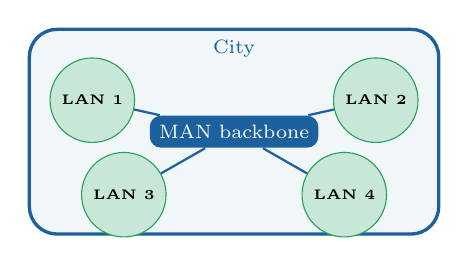
\begin{tikzpicture}
        \draw[ocean,very thick,rounded corners=10pt,fill=ocean!6] (-2.6,-1.3) rectangle (2.6,1.3);
        \node[font=\scriptsize,text=ocean] at (0,1.05) {City};
        \node[fill=ocean,text=white,font=\scriptsize,rounded corners] (b) at (0,0) {MAN backbone};
        \foreach \p/\l in {(-1.8,0.4)/LAN 1,(1.8,0.4)/LAN 2,(-1.4,-0.8)/LAN 3,(1.4,-0.8)/LAN 4}{
          \node[fill=leaf!25,draw=leaf,circle,font=\tiny\bfseries,minimum size=8mm] (n) at \p {\l};
          \draw[ocean,thick] (b) -- (n);
        }
      \end{tikzpicture}\\[1mm]
      \begin{itemize}\scriptsize
        \item Connects the LANs of a company's offices across a city
        \item Private, or leased from a telephone / cable company
        \item E.g. \textbf{SMDS}, cable TV networks
      \end{itemize}
    \end{column}
    \begin{column}{0.49\textwidth}
      \centering\textbf{\textcolor{grape}{WAN: country, continent, world}}\\[2mm]
      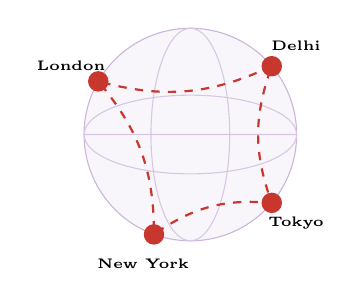
\begin{tikzpicture}
        \draw[grape!40,fill=grape!5] (0,0) circle (1.35);
        \draw[grape!30] (0,0) ellipse (1.35 and 0.5) (0,0) ellipse (0.5 and 1.35) (-1.35,0) -- (1.35,0);
        \foreach \a/\l in {40/Delhi,150/London,250/New York,320/Tokyo}{
          \fill[brick] (\a:1.35) circle (1.3mm);
          \node[font=\tiny\bfseries] at (\a:1.75) {\l};
        }
        \draw[brick,thick,dashed] (40:1.35) to[bend left=20] (150:1.35) to[bend left=20] (250:1.35) to[bend left=20] (320:1.35) to[bend left=20] (40:1.35);
      \end{tikzpicture}\\[1mm]
      \begin{itemize}\scriptsize
        \item Long-distance transmission of data, voice, image, video
        \item Uses public, leased or private \textbf{communication devices}
        \item Wholly owned by one company: an \textbf{enterprise network}
      \end{itemize}
    \end{column}
  \end{columns}
\end{frame}

% ------------------------------------------------------------
\begin{frame}{LAN vs. MAN vs. WAN}
  \centering
  \renewcommand{\arraystretch}{1.5}
  \begin{tabular}{>{\bfseries}l >{\columncolor{leaf!10}}c >{\columncolor{ocean!10}}c >{\columncolor{grape!10}}c}
    \toprule
    \rowcolor{navy}\textcolor{white}{Feature} & \textcolor{white}{\textbf{LAN}} & \textcolor{white}{\textbf{MAN}} & \textcolor{white}{\textbf{WAN}}\\
    \midrule
    Coverage      & Office, building, campus & Entire city & Country, continent, world\\
    Distance      & A few km & Tens of km & Unlimited\\
    Ownership     & Private & Private or public company & Public, leased or private\\
    Speed         & High (100 Mbps--Gbps) & Medium--high & Lower, varies\\
    Hardware      & Own cabling & Cable / telephone lines & Communication carriers\\
    Example       & College computer lab & City-wide cable network & The Internet backbone\\
    \bottomrule
  \end{tabular}
\end{frame}

% ------------------------------------------------------------
\begin{frame}{Internetworks: internet vs. Internet}
  \begin{columns}[c]
    \begin{column}{0.55\textwidth}
      \centering
      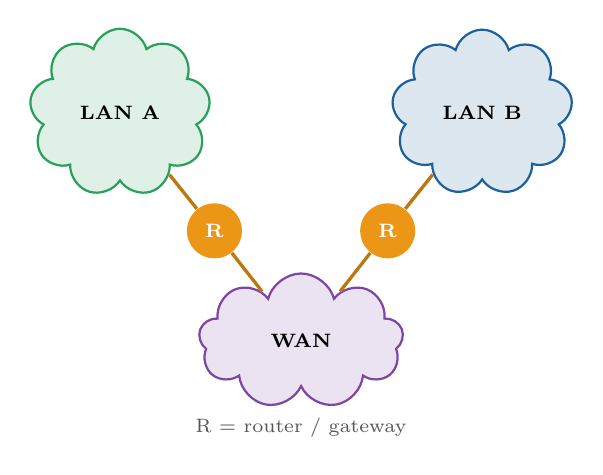
\begin{tikzpicture}
        \node[cloud,cloud puffs=9,draw=leaf,fill=leaf!15,thick,minimum width=2.3cm,minimum height=1.3cm,font=\scriptsize\bfseries] (n1) at (0,1.6) {LAN A};
        \node[cloud,cloud puffs=9,draw=ocean,fill=ocean!15,thick,minimum width=2.3cm,minimum height=1.3cm,font=\scriptsize\bfseries] (n2) at (4.6,1.6) {LAN B};
        \node[cloud,cloud puffs=9,draw=grape,fill=grape!15,thick,minimum width=2.6cm,minimum height=1.4cm,font=\scriptsize\bfseries] (n3) at (2.3,-1.3) {WAN};
        \node[circle,fill=amber,text=white,font=\scriptsize\bfseries,minimum size=7mm] (r1) at (1.2,0.1) {R};
        \node[circle,fill=amber,text=white,font=\scriptsize\bfseries,minimum size=7mm] (r2) at (3.4,0.1) {R};
        \draw[very thick,amber!80!black] (n1) -- (r1) -- (n3);
        \draw[very thick,amber!80!black] (n2) -- (r2) -- (n3);
        \node[tag] at (2.3,-2.4) {R = router / gateway};
      \end{tikzpicture}
    \end{column}
    \begin{column}{0.43\textwidth}
      \begin{itemize}\setlength{\itemsep}{4pt}\small
        \item When two or more networks are connected, they form an \textbf{internetwork}
        \item They are joined by \textbf{routers and gateways}
      \end{itemize}
      \vspace{2mm}
      \begin{block}{Do not confuse}
        \small
        \textbf{internet} (lowercase $i$): any interconnection of networks\\[3pt]
        \textbf{Internet} (uppercase $I$): the specific \textbf{worldwide} network
      \end{block}
    \end{column}
  \end{columns}
\end{frame}


\begin{frame}{Layered Tasks: The Postal Analogy}
  \centering
  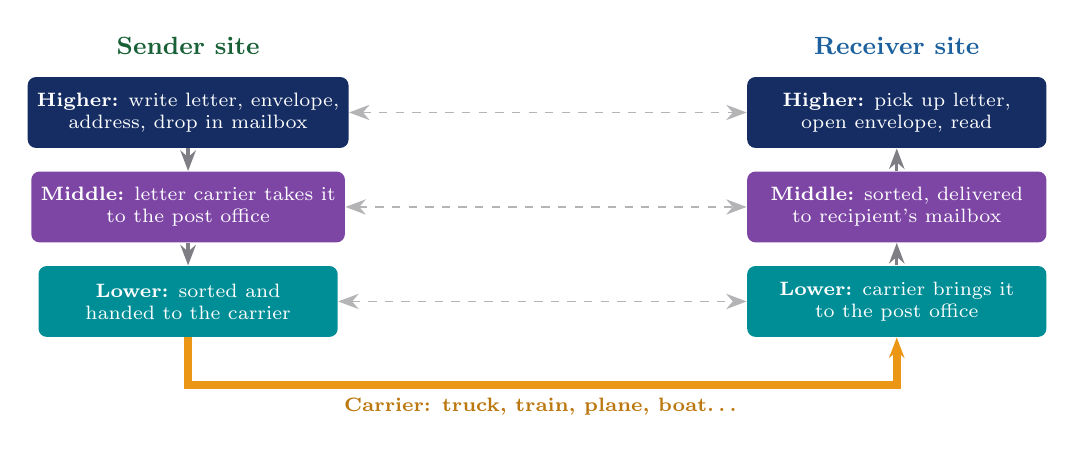
\begin{tikzpicture}
    \node[font=\small\bfseries,text=leaf!60!black] at (0,2.25) {Sender site};
    \node[font=\small\bfseries,text=ocean] at (9,2.25) {Receiver site};
    \node[lay=navy]  (s3) at (0,1.4)  {\textbf{Higher:} write letter, envelope,\\address, drop in mailbox};
    \node[lay=grape] (s2) at (0,0.2)  {\textbf{Middle:} letter carrier takes it\\to the post office};
    \node[lay=aqua]  (s1) at (0,-1.0) {\textbf{Lower:} sorted and\\handed to the carrier};
    \node[lay=navy]  (r3) at (9,1.4)  {\textbf{Higher:} pick up letter,\\open envelope, read};
    \node[lay=grape] (r2) at (9,0.2)  {\textbf{Middle:} sorted, delivered\\to recipient's mailbox};
    \node[lay=aqua]  (r1) at (9,-1.0) {\textbf{Lower:} carrier brings it\\to the post office};
    \draw[->,very thick,ink!60] (s3) -- (s2); \draw[->,very thick,ink!60] (s2) -- (s1);
    \draw[->,very thick,ink!60] (r1) -- (r2); \draw[->,very thick,ink!60] (r2) -- (r3);
    \draw[->,line width=3pt,amber] (s1.south) -- ++(0,-0.6) -- node[below,font=\scriptsize\bfseries,text=amber!80!black]{Carrier: truck, train, plane, boat\dots} ++(9,0) -- (r1.south);
    \foreach \a/\b in {s3/r3,s2/r2,s1/r1} \draw[<->,dashed,ink!35] (\a) -- (\b);
  \end{tikzpicture}
  \vspace{2mm}

  {\small Each layer at the sender \textbf{uses the services of the layer below it}. The receiver does the tasks in \textbf{reverse order}.}
\end{frame}


% ------------------------------------------------------------
\begin{frame}{The ISO: Who Makes the Standards?}
  \begin{columns}[c]
    \begin{column}{0.5\textwidth}
      \centering
      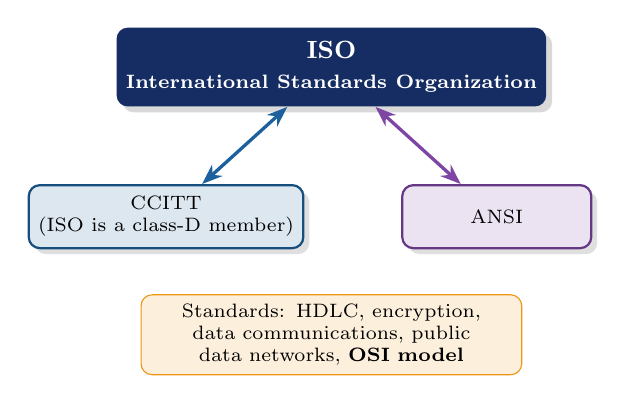
\begin{tikzpicture}
        \node[solid box=navy,minimum width=40mm,minimum height=10mm] (iso) at (0,0) {ISO\\\scriptsize International Standards Organization};
        \node[box=ocean,minimum width=24mm,font=\scriptsize] (itu) at (-2.1,-1.9) {CCITT\\(ISO is a class-D member)};
        \node[box=grape,minimum width=24mm,font=\scriptsize] (ansi) at (2.1,-1.9) {ANSI};
        \draw[<->,very thick,ocean] (iso) -- (itu);
        \draw[<->,very thick,grape] (iso) -- (ansi);
        \node[fill=amber!15,draw=amber,rounded corners,font=\scriptsize,text width=46mm,align=center] at (0,-3.4)
          {Standards: HDLC, encryption, data communications, public data networks, \textbf{OSI model}};
      \end{tikzpicture}
    \end{column}
    \begin{column}{0.48\textwidth}
      \begin{itemize}\setlength{\itemsep}{5pt}\small
        \item A \textbf{voluntary organization} of national standards committees from each member country
        \item Coordinates its activities with \textbf{CCITT} on common issues
        \item Works with CCITT and \textbf{ANSI} through subcommittees and working groups
        \item Best-known product: the \hl{Open Systems Interconnection (OSI)} model
      \end{itemize}
    \end{column}
  \end{columns}
\end{frame}

% ------------------------------------------------------------
\begin{frame}{The Internet Model (TCP/IP Protocol Suite)}
  \begin{columns}[c]
    \begin{column}{0.4\textwidth}
      \centering
      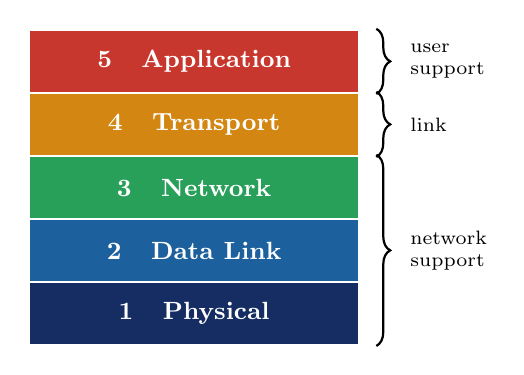
\begin{tikzpicture}[node distance=0pt]
        \foreach \n/\t/\c [count=\i] in {5/Application/brick,4/Transport/amber!90!black,3/Network/leaf,2/Data Link/ocean,1/Physical/navy}
          \node[layer=\c,minimum width=42mm,minimum height=8mm] (L\n) at (0,-\i*0.8) {\n \quad \t};
        \draw[decorate,decoration={brace,amplitude=5pt},thick] ([xshift=2mm]L5.north east) -- node[right=3mm,font=\scriptsize,align=left]{user\\support} ([xshift=2mm]L5.south east);
        \draw[decorate,decoration={brace,amplitude=5pt},thick] ([xshift=2mm]L4.north east) -- node[right=3mm,font=\scriptsize,align=left]{link} ([xshift=2mm]L4.south east);
        \draw[decorate,decoration={brace,amplitude=5pt},thick] ([xshift=2mm]L3.north east) -- node[right=3mm,font=\scriptsize,align=left]{network\\support} ([xshift=2mm]L1.south east);
      \end{tikzpicture}
    \end{column}
    \begin{column}{0.58\textwidth}
      \begin{itemize}\setlength{\itemsep}{4pt}\small
        \item A \textbf{five-layer} model; also called the \textbf{TCP/IP protocol suite}
        \item Each layer defines a \textbf{family of functions} distinct from the others
        \item Layers \textbf{1--3}: network support (physically moving data)
        \item Layer \textbf{5}: user support (interoperability between software)
        \item Layer \textbf{4} links the two groups and ensures the lower layers deliver data in a form the upper layers can use
      \end{itemize}
      \vspace{2mm}
      \begin{block}{Design goal}
        \small A \textbf{comprehensive and flexible} architecture.
      \end{block}
    \end{column}
  \end{columns}
\end{frame}

% ------------------------------------------------------------
\begin{frame}{A Message Travels from Device A to Device B}
  \centering
  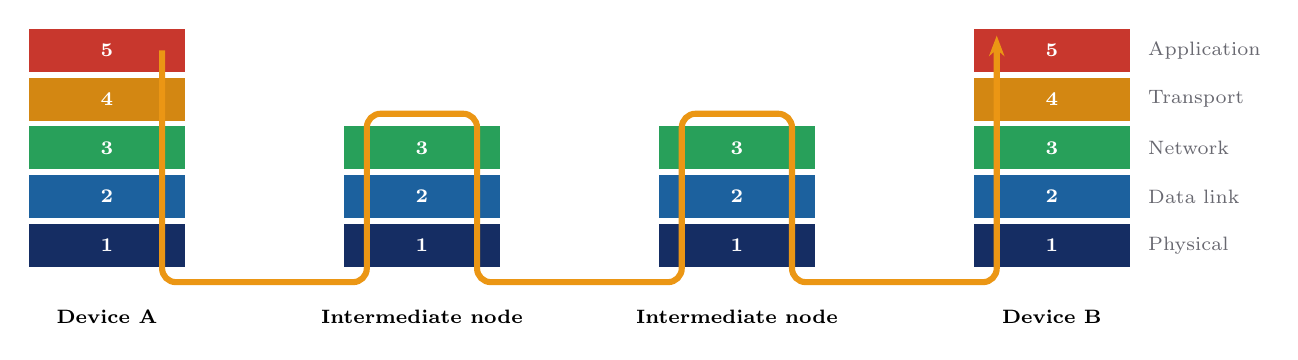
\begin{tikzpicture}[x=1cm,y=0.62cm]
    \def\cols{{"navy","ocean","leaf","amber!90!black","brick"}}
    % Device A and B: 5 layers; intermediate nodes: 3 layers
    \foreach \X/\n/\lab in {0/5/Device A,4/3/Intermediate node,8/3/Intermediate node,12/5/Device B}{
      \foreach \i in {1,...,\n}{
        \pgfmathsetmacro{\c}{\cols[\i-1]}
        \node[fill=\c,text=white,font=\scriptsize\bfseries,minimum width=20mm,minimum height=5.6mm,draw=white] at (\X,\i) {\i};
      }
      \node[font=\scriptsize\bfseries] at (\X,-0.45) {\lab};
    }
    \draw[amber,line width=2.2pt,->,rounded corners=5pt]
      (0.7,5) -- (0.7,0.25) -- (3.3,0.25) -- (3.3,3.7) -- (4.7,3.7) -- (4.7,0.25) -- (7.3,0.25) -- (7.3,3.7) -- (8.7,3.7) -- (8.7,0.25)
      -- (11.3,0.25) -- (11.3,5.3);
    \foreach \i/\t in {5/Application,4/Transport,3/Network,2/Data link,1/Physical}
      \node[font=\scriptsize,anchor=west,text=ink!70] at (13.1,\i) {\t};
  \end{tikzpicture}
  \vspace{2mm}

  {\small Intermediate nodes (routers) usually involve \textbf{only the first three layers}. Between machines, layer $x$ on one machine communicates with layer $x$ on the other using a \textbf{protocol}.}
\end{frame}

% ------------------------------------------------------------
\begin{frame}{Peer-to-Peer Processes and Encapsulation}
  \begin{columns}[c]
    \begin{column}{0.56\textwidth}
      \centering
      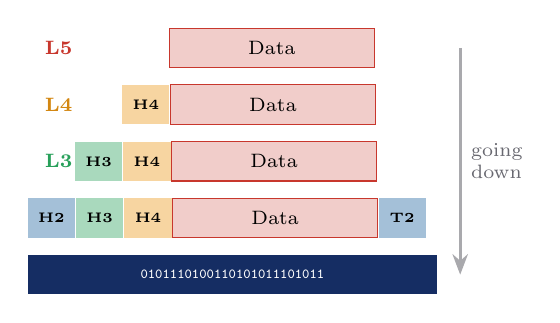
\begin{tikzpicture}[y=0.72cm]
        \foreach \i/\c/\h in {5/brick/,4/amber!90!black/H4,3/leaf/H3,2/ocean/H2,1/navy/}{
          \node[font=\scriptsize\bfseries,text=\c,anchor=east] at (-0.2,\i) {L\i};
        }
        % application data
        \node[fill=brick!25,draw=brick,minimum width=26mm,minimum height=5mm,font=\scriptsize,anchor=west] at (0.9,5) {Data};
        \node[fill=amber!40,minimum width=6mm,minimum height=5mm,font=\tiny\bfseries,anchor=west] (h4) at (0.3,4) {H4};
        \node[fill=brick!25,draw=brick,minimum width=26mm,minimum height=5mm,font=\scriptsize,anchor=west] at (h4.east) {Data};
        \node[fill=leaf!40,minimum width=6mm,minimum height=5mm,font=\tiny\bfseries,anchor=west] (h3) at (-0.3,3) {H3};
        \node[fill=amber!40,minimum width=6mm,minimum height=5mm,font=\tiny\bfseries,anchor=west] (h3b) at (h3.east) {H4};
        \node[fill=brick!25,draw=brick,minimum width=26mm,minimum height=5mm,font=\scriptsize,anchor=west] (d3) at (h3b.east) {Data};
        \node[fill=ocean!40,minimum width=6mm,minimum height=5mm,font=\tiny\bfseries,anchor=west] (h2) at (-0.9,2) {H2};
        \node[fill=leaf!40,minimum width=6mm,minimum height=5mm,font=\tiny\bfseries,anchor=west] (x1) at (h2.east) {H3};
        \node[fill=amber!40,minimum width=6mm,minimum height=5mm,font=\tiny\bfseries,anchor=west] (x2) at (x1.east) {H4};
        \node[fill=brick!25,draw=brick,minimum width=26mm,minimum height=5mm,font=\scriptsize,anchor=west] (x3) at (x2.east) {Data};
        \node[fill=ocean!40,minimum width=6mm,minimum height=5mm,font=\tiny\bfseries,anchor=west] at (x3.east) {T2};
        \node[fill=navy,text=white,minimum width=52mm,minimum height=5mm,font=\tiny\ttfamily,anchor=west] at (-0.9,1) {0101110100110101011101011};
        \draw[->,very thick,ink!40] (4.6,5) -- (4.6,1) node[midway,right,font=\scriptsize,text=ink!70,align=left]{going\\down};
      \end{tikzpicture}
    \end{column}
    \begin{column}{0.42\textwidth}
      \begin{itemize}\setlength{\itemsep}{4pt}\small
        \item \textbf{Peer-to-peer processes}: the processes at the same layer on each machine
        \item Each sending layer \textbf{adds its own header} (and sometimes a trailer) and passes the package down
        \item At layer 1 everything becomes a \textbf{bit stream}
        \item The receiver \textbf{unwraps} layer by layer
        \item \textbf{Interfaces} between adjacent layers define what services each layer offers
      \end{itemize}
    \end{column}
  \end{columns}
\end{frame}

% ------------------------------------------------------------
\begin{frame}{Layers 1 \& 2: Physical and Data Link}
  \begin{columns}[T]
    \begin{column}{0.48\textwidth}
      
\begin{tikzpicture}
        \node[fill=navy,text=white,rounded corners=4pt,minimum width=62mm,minimum height=9mm,font=\bfseries] {1 \;\; Physical Layer};
      \end{tikzpicture}\\[1mm]
      {\small Transmits a \textbf{bit stream} over a physical medium.}
      \begin{itemize}\scriptsize\setlength{\itemsep}{2pt}
        \item \textbf{Interface \& media}: mechanical and electrical specifications
        \item \textbf{Representation of bits}: encode bits as electrical or optical signals
        \item \textbf{Data rate}: bits sent per second
        \item \textbf{Synchronization}: sender and receiver clocks agree
      \end{itemize}
      \centering
      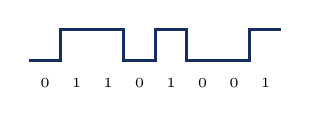
\begin{tikzpicture}[x=4mm,y=4mm]
        \draw[navy,very thick] (0,0) -- (1,0) -- (1,1) -- (3,1) -- (3,0) -- (4,0) -- (4,1) -- (5,1) -- (5,0) -- (7,0) -- (7,1) -- (8,1);
        \foreach \b [count=\i from 0] in {0,1,1,0,1,0,0,1} \node[font=\tiny] at (\i+0.5,-0.7) {\b};
      \end{tikzpicture}
    \end{column}
    \begin{column}{0.48\textwidth}
      
\begin{tikzpicture}
        \node[fill=ocean,text=white,rounded corners=4pt,minimum width=62mm,minimum height=9mm,font=\bfseries] {2 \;\; Data Link Layer};
      \end{tikzpicture}\\[1mm]
      {\small Turns the raw physical layer into a \textbf{reliable link}.}
      \begin{itemize}\scriptsize\setlength{\itemsep}{2pt}
        \item \textbf{Framing}: divides the bit stream into \textbf{frames}
        \item \textbf{Physical addressing}: header holds sender and receiver addresses
        \item \textbf{Flow control}: does not overwhelm a slow receiver
        \item \textbf{Error control}: detects and retransmits damaged or lost frames (trailer)
        \item \textbf{Access control}: decides which device uses the link
      \end{itemize}
      \centering
      \begin{tikzpicture}
        \node[fill=ocean!40,minimum height=5mm,font=\tiny\bfseries] (a) {Header};
        \node[fill=ocean!10,draw=ocean,minimum width=20mm,minimum height=5mm,font=\tiny,right=0pt of a] (b) {Data from layer 3};
        \node[fill=ocean!40,minimum height=5mm,font=\tiny\bfseries,right=0pt of b] {Trailer};
      \end{tikzpicture}
    \end{column}
  \end{columns}
\end{frame}

% ------------------------------------------------------------
\begin{frame}{Layers 3 \& 4: Network and Transport}
  \begin{columns}[T]
    \begin{column}{0.48\textwidth}
      \begin{tikzpicture}
        \node[fill=leaf,text=white,rounded corners=4pt,minimum width=62mm,minimum height=9mm,font=\bfseries] {3 \;\; Network Layer};
      \end{tikzpicture}\\[1mm]
      {\small \textbf{Source-to-destination} delivery of a \textbf{packet}, possibly across many networks.}
      \begin{itemize}\scriptsize\setlength{\itemsep}{2pt}
        \item \textbf{Logical addressing}: addresses that work beyond the local network (e.g. IP address)
        \item \textbf{Routing}: \textbf{routers} forward packets to their final destination
      \end{itemize}
      \centering
      \begin{tikzpicture}
        \foreach \x/\l/\s/\k in {0/A/90/a,1.5/R/50/b,3/R/50/c,4.5/B/90/d}
          \node[circle,fill=leaf!\s!black,text=white,font=\scriptsize\bfseries,minimum size=7mm] (n\k) at (\x,0) {\l};
        \draw[->,thick,leaf!70!black] (na) -- (nb); \draw[->,thick,leaf!70!black] (nb) -- (nc); \draw[->,thick,leaf!70!black] (nc) -- (nd);
        \node[tag] at (2.25,-0.6) {host to host};
      \end{tikzpicture}
    \end{column}
    \begin{column}{0.48\textwidth}
      \begin{tikzpicture}
        \node[fill=amber!90!black,text=white,rounded corners=4pt,minimum width=62mm,minimum height=9mm,font=\bfseries] {4 \;\; Transport Layer};
      \end{tikzpicture}\\[1mm]
      {\small \textbf{Process-to-process} delivery of the \textbf{entire message}, in order and intact.}
      \begin{itemize}\scriptsize\setlength{\itemsep}{2pt}
        \item \textbf{Port addressing}: reach the right \emph{program} on a computer
        \item \textbf{Segmentation \& reassembly}: segments carry sequence numbers
        \item \textbf{Connection control}: connectionless or connection-oriented
        \item \textbf{Flow \& error control}: end to end, not per link
      \end{itemize}
      \centering
      \begin{tikzpicture}
        \foreach \i in {1,2,3} \node[fill=amber!30,draw=amber!90!black,font=\tiny\bfseries,minimum width=10mm] at (\i*1.2,0) {seg \i};
        \node[tag] at (2.4,-0.5) {numbered segments};
      \end{tikzpicture}
    \end{column}
  \end{columns}
\end{frame}

% ------------------------------------------------------------
\begin{frame}{Layer 5: Application Layer}
  \begin{columns}[c]
    \begin{column}{0.5\textwidth}
      \centering
      \begin{tikzpicture}
        \node[circle,fill=brick,text=white,font=\bfseries,minimum size=20mm,align=center,drop shadow] (c) at (0,0) {Application\\Layer};
        \foreach \a/\t/\c in {90/Mail services/ocean,0/File transfer\\\& access/leaf,270/Remote login/grape,180/World Wide\\Web/amber!90!black}{
          \node[solid box=\c,minimum width=24mm,font=\scriptsize\bfseries] (s\a) at (\a:2.6) {\t};
          \draw[very thick,\c] (c) -- (s\a);
        }
      \end{tikzpicture}
    \end{column}
    \begin{column}{0.48\textwidth}
      Lets the \textbf{user} (a person or software) \textbf{access the network}. It provides user interfaces and support for services:
      \vspace{2mm}
      \begin{itemize}\small\setlength{\itemsep}{3pt}
        \item \textcolor{ocean}{\textbf{Mail services}}: e-mail forwarding and storage
        \item \textcolor{leaf!70!black}{\textbf{File transfer \& access}}: retrieve and manage files on a remote host
        \item \textcolor{grape}{\textbf{Remote login}}: log in and use a remote computer
        \item \textcolor{amber!80!black}{\textbf{WWW}}: the most common application today
      \end{itemize}
    \end{column}
  \end{columns}
\end{frame}

% ------------------------------------------------------------
\begin{frame}{The OSI Model: Seven Layers}
  \begin{columns}[c]
    \begin{column}{0.44\textwidth}
      \centering
      \begin{tikzpicture}
        \foreach \n/\t/\c [count=\i] in {7/Application/brick,6/Presentation/grape,5/Session/grape!70!ocean,4/Transport/amber!90!black,3/Network/leaf,2/Data Link/ocean,1/Physical/navy}
          \node[layer=\c,minimum width=46mm,minimum height=7mm] at (0,-\i*0.72) {\n \quad \t};
        \node[font=\scriptsize,text=ink!60] at (0,-6.0) {``\textbf{A}ll \textbf{P}eople \textbf{S}eem \textbf{T}o \textbf{N}eed \textbf{D}ata \textbf{P}rocessing''};
      \end{tikzpicture}
    \end{column}
    \begin{column}{0.54\textwidth}
      \begin{itemize}\setlength{\itemsep}{4pt}\small
        \item \textbf{Open Systems Interconnection} model by the \textbf{ISO}
        \item A \textbf{theoretical} model showing how a protocol stack \emph{should} be built
        \item Never seriously implemented as a real protocol stack
        \item Adds \textbf{two extra layers} to the Internet model:
      \end{itemize}
      \vspace{1mm}
      \begin{block}{Session layer (5)}
        \scriptsize The network \textbf{dialog controller}: establishes, maintains and synchronizes interaction.
      \end{block}
      \begin{block}{Presentation layer (6)}
        \scriptsize Syntax and semantics: \textbf{translation, encryption/decryption, compression}.
      \end{block}
    \end{column}
  \end{columns}
\end{frame}

% ------------------------------------------------------------
\begin{frame}{OSI vs. TCP/IP: Side by Side}
  \centering
  \begin{tikzpicture}
    \node[font=\bfseries,text=navy] at (0,0.55) {OSI (7 layers)};
    \node[font=\bfseries,text=navy] at (7,0.55) {Internet / TCP/IP (5 layers)};
    \foreach \n/\t/\c [count=\i] in {7/Application/brick,6/Presentation/grape,5/Session/grape!70!ocean,4/Transport/amber!90!black,3/Network/leaf,2/Data Link/ocean,1/Physical/navy}
      \node[layer=\c,minimum width=42mm,minimum height=5.8mm] (o\n) at (0,-\i*0.6+0.1) {\t};
    \node[layer=brick,minimum width=42mm,minimum height=17.9mm,fill=brick] (t5) at (7,-1.1) {Application};
    \foreach \n/\t/\c [count=\i from 4] in {4/Transport/amber!90!black,3/Network/leaf,2/Data Link/ocean,1/Physical/navy}
      \node[layer=\c,minimum width=42mm,minimum height=5.8mm] (t\n) at (7,-\i*0.6+0.1) {\t};
    \draw[dashed,thick,ink!40] (o7.north east) -- (t5.north west);
    \draw[dashed,thick,ink!40] (o5.south east) -- (t5.south west);
    \foreach \n in {4,3,2,1} \draw[<->,thick,ink!40] (o\n.east) -- (t\n.west);
    \node[fill=amber!15,draw=amber,rounded corners,font=\scriptsize,text width=24mm,align=center] at (3.5,-1.1) {Session and presentation \textbf{merged into application}};
  \end{tikzpicture}
  \vspace{1mm}
  \begin{block}{Why the five-layer model is used more}
    \small Session and presentation duties are now handled by other layers: encryption happens at \textbf{several} layers, compression at the application layer.
  \end{block}
\end{frame}

% ------------------------------------------------------------
\begin{frame}{The Internet Activities Board (IAB)}
  \begin{columns}[c]
    \begin{column}{0.5\textwidth}
      \centering
      \begin{tikzpicture}[node distance=9mm]
        \node[solid box=navy,minimum width=46mm,minimum height=10mm] (iab) {Internet Activities Board\\(IAB)};
        \node[box=ocean,minimum width=24mm,font=\scriptsize,below left=9mm and -12mm of iab] (tf) {Task forces};
        \node[box=grape,minimum width=24mm,font=\scriptsize,below right=9mm and -12mm of iab] (gr) {Working groups};
        \draw[->,very thick,navy] (iab) -- (tf); \draw[->,very thick,navy] (iab) -- (gr);
        \node[solid box=leaf,minimum width=46mm,below=22mm of iab] (tcp) {TCP/IP standards};
        \draw[->,very thick,ocean] (tf) -- (tcp); \draw[->,very thick,grape] (gr) -- (tcp);
        \node[tag,right=1mm of tf,xshift=6mm,yshift=-8mm] {};
      \end{tikzpicture}
    \end{column}
    \begin{column}{0.48\textwidth}
      \begin{itemize}\setlength{\itemsep}{5pt}\small
        \item One of the most successful bodies for setting \textbf{data transfer standards} in the Internet arena
        \item Has \textbf{overall authority} for these activities
        \item Several task forces and groups \textbf{define new protocols} and \textbf{improve existing ones}
        \item Best-known result: the widely used \hl{TCP/IP} suite
      \end{itemize}
    \end{column}
  \end{columns}
\end{frame}

% ------------------------------------------------------------
\begin{frame}{Bridge to the Course: Security at Every Layer}
  \centering
  \begin{tikzpicture}
    \foreach \n/\t/\c/\s/\m [count=\i] in {
      5/Application/brick/PGP\comma{} S\slash MIME\comma{} Kerberos\comma{} SET/Modules 11--12,
      4/Transport/amber!90!black/SSL\slash TLS (secure web)/Module 12,
      3/Network/leaf/IPSec (AH\comma{} ESP)/Module 12,
      2/Data Link/ocean/Link encryption/--,
      1/Physical/navy/Physical protection of cables/--}
    {
      \node[layer=\c,minimum width=38mm,minimum height=8mm] (L\i) at (0,-\i*0.9) {\n \quad \t};
      \pic[scale=0.5] at (2.6,-\i*0.9) {lock=\c};
      \node[anchor=west,font=\small] at (3.1,-\i*0.9) {\s};
      \node[anchor=west,font=\scriptsize,text=ink!60] at (9.2,-\i*0.9) {\m};
    }
  \end{tikzpicture}
  \vspace{3mm}
  \begin{exampleblock}{Big picture}
    \small The \textbf{cryptography} of Lesson 1 is the tool; the \textbf{layers} of Lesson 2 are where we apply it. The rest of the course builds on both.
  \end{exampleblock}
\end{frame}

% ------------------------------------------------------------
\begin{frame}{Module 1 Summary}
  \begin{columns}[T]
    \begin{column}{0.49\textwidth}
      \begin{block}{Lesson 1: Introduction to Network Security}
        \small
        \begin{itemize}\setlength{\itemsep}{1pt}
          \item CIA goals and the three aspects
          \item Interruption, interception, modification, fabrication
          \item Cryptology = cryptography + cryptanalysis
          \item 3 dimensions of cryptosystems
          \item Brute force and 6 cryptanalytic attacks
        \end{itemize}
      \end{block}
    \end{column}
    \begin{column}{0.49\textwidth}
      \begin{exampleblock}{Lesson 2: Network Models}
        \small
        \begin{itemize}\setlength{\itemsep}{1pt}
          \item LAN, MAN, WAN and internetworks
          \item Layered tasks (postal analogy)
          \item ISO and the OSI 7-layer model
          \item TCP/IP 5-layer Internet model
          \item Duties of each layer
          \item IAB and Internet standards
        \end{itemize}
      \end{exampleblock}
    \end{column}
  \end{columns}
  \vspace{1mm}
  \begin{alertblock}{Review questions}
    \small
    1.~Discuss cryptography in brief. \quad
    2.~Define cryptanalysis. \quad
    3.~Explain different categories of networks. \quad
    4.~Differentiate between the OSI and TCP/IP models.
  \end{alertblock}
\end{frame}

% ------------------------------------------------------------
\begin{frame}{References}
  \begin{enumerate}\setlength{\itemsep}{8pt}
    \item William Stallings, \emph{Cryptography and Network Security}, PHI Publishers.
    \item Charlie Kaufman, Radia Perlman, \emph{Network Security}, Pearson Education.
    \item Bruce Schneier, \emph{Applied Cryptography}, John Wiley \& Sons.
    \item Roberta Bragg, \emph{Network Security: The Complete Reference}, TMH.
  \end{enumerate}
  \vspace{6mm}
  \centering
  \begin{tikzpicture}
    \node[fill=navy,text=white,rounded corners=8pt,inner sep=10pt,font=\Large\bfseries,drop shadow] {Thank You! \; Questions?};
  \end{tikzpicture}
\end{frame}

\end{document}
